\documentclass{article}

\usepackage{graphicx}

\usepackage{color}

\usepackage{amsmath, amssymb, amsthm}

\usepackage{float}

\usepackage{caption}
 
\usepackage{algorithmicx, algorithm, algpseudocode}
\floatname{algorithm}{Algorithm}
 
%\usepackage[noline,boxruled,commentsnumbered,linesnumbered,titlenumbered]{algorithm2e}
 
\title{discrete element code}
\author{
  Konstantinos Krestenitis
  \and
  Tobias Weinzierl
  \and
  Tomasz Koziara\thanks{
    School of Engineering and Computing Sciences, Durham University,
    DH1 3LE Durham, UK,
    konstantinos.krestenitis@durham.ac.uk
  }
}
\date{\today}

\newcommand{\DeltaSoftware}{\texttt{Delta} $\Delta$}

 \newenvironment{observation}[1][Observation]{\vspace{0.2cm}\noindent\textbf{#1.}\
 }{\vspace{0.2cm}}



\begin{document}
\maketitle

\marginpar{\footnotesize We should again discuss whether we can get Jon
on-board}

\section{Introduction}

\marginpar{\footnotesize What is DEM. Why does DEM matter (application areas)?}
Lorem ipsum. Lorem ipsum. Lorem ipsum. Lorem ipsum. Lorem ipsum. Lorem ipsum.
Lorem ipsum. Lorem ipsum. Lorem ipsum. Lorem ipsum. Lorem ipsum. Lorem ipsum. 

\marginpar{\footnotesize There are two important shortcomings of many codes:
only spheres and too few of them. Furthermore, many codes suffer if spheres
are of different orders of magnitudes. Why does it make sense to tackle this?}
Lorem ipsum.
Lorem ipsum.
Lorem ipsum. Lorem ipsum. Lorem ipsum. Lorem ipsum.
Lorem ipsum. Lorem ipsum. Lorem ipsum. Lorem ipsum. Lorem ipsum. Lorem ipsum. 

\marginpar{\footnotesize Major objective/contribution of this paper.}
Upscaling a DEM code with respect to particle count and machine size 
challenges the objective to work with triangulated particles from a vast range
of particle sizes.
DEM codes spend a majority of their compute time in collision detection.
\marginpar{\footnotesize Tomek: citation.} 
This phase becomes significantly more complicated if we switch from
sphere-to-sphere checks to the comparison of billions of triangles.
Geometric comparisons suffer from poor SIMDability if realised
straightforwardly.
Multiple contact points between any pair of particles may exist, and it is
impossible to predict statically how this computational workload distributes
between ranks if particles are distributed among ranks. 
The distribution itself is non-trivial if there are particles from a vast range
of scales, which in turn again makes the contact point relation more complicated
than for particle sets of (roughly) the same size.
Finally, the amount of data to be exchanged per particle is higher
than for spherical data where a centre and a radius describe the object of interest. 
The computational work thus increases significantly with any increase of
particle counts.
The scalability of this computational work in turn is not given by construction.
The present paper introduces realisation idioms of a triangle-based DEM code
that fuses efficiency and scalability on all levels of the machine architecture spanning from
vectorisation and memory access characteristics over manycore to inter-node
data exchange.
It shows that the upcoming massively parallel era will allow us to
simulate non-sperical DEM formulations with unpreceded speed.   

\marginpar{\footnotesize What do we do and how does it differ/fit to others'
work?}
Lorem ipsum. Lorem ipsum. Lorem ipsum. Lorem ipsum. Lorem ipsum. Lorem ipsum.
Lorem ipsum. Lorem ipsum. Lorem ipsum. Lorem ipsum. Lorem ipsum. Lorem ipsum. 

\marginpar{\footnotesize Shortcomings and limitations of the present approach.}
Lorem ipsum. Lorem ipsum. Lorem ipsum. Lorem ipsum. Lorem ipsum. Lorem ipsum.
Lorem ipsum. Lorem ipsum. Lorem ipsum. Lorem ipsum. Lorem ipsum. Lorem ipsum. 


- Non-spherical particles reduce efficiency significantly [78,104] in Samiei
- Analytical shape functions besides spheres [41,56,61,118] in Semiei und er
selbst
- Generic shape composition with spheres [75] und Samiei selber


\marginpar{\footnotesize Structure of work.}
The remainder of the paper is organised as follows: 
We start from a brief sketch the overall DEM simulation with
explicit time stepping in Section \ref{section:algorithm}. 
A multiscale grid meta data structure (Section \ref{section:grid}) helps us to
reduce the algorithms complexity to linear.
Starting from this, the main part of the contribution studies a proper data
layout of particle and collision data (Section \ref{section:vectorisation}) that is well-suited for
vectorisation, allows us to exploit multi- and manycore
architectures in various ways (Section \ref{section:shared-memory}) as well as
classic parallel architectures via MPI and domain decomposition (Section
\ref{section:domain-decomposition}).
In Section \ref{section:benchmarks}, we use all algorithmic ingredients to run some benchmarks
that reveal the potential and impact of a technology supporting non-spherical
particles efficiently, before we present performance studies (Section
\ref{section:results}).
A brief summary and an outlook close the discussion.

\section{Algorithm outline}
\label{section:algorithm}

contact 
forces
dynamics/rotation/timestep
 
\begin{algorithm}
 
   Blueprint of explicit DEM code's overall structure.
 
 \label{algorithm:dem-blueprint}
% \SetAlgoNoLine
 \begin{algorithmic}[1]
   \For{$t < T$}
   
	\For{i = 0 to N triangles}

		\For {j = i+1 to N triangles}
				
			\State $distance = TTD(i,j)$
				
			\If{(distance $<$ margin) AND ParticleID(i) != ParticleID(j)}

				\State $contact(PID(i)).add(point, normal)$

			\EndIf
			
		\EndFor
			
	\EndFor


	\For{z = 0 to NB particles}

		\For {k = 0 to contacts(z).size()}

			\State $force = granular(velocity(z), position(z), contacts(z).getcontact(k))$

		\EndFor
	
	\EndFor    
    
     \State $t \gets t + \Delta t$
   \EndFor   

 \end{algorithmic}
\end{algorithm} 


We focus on DEM with explicit time stepping (Algorithm \ref{algorithm:dem-blueprint}). 
A straightforward implementation consists of one outer time stepping loop
hosting three inner loops. 
The first inner loop detects contact points between particles' triangles and
check each triangle vs.~the others.
It thus has to loop over the particles.
The second loop runs over these contact points and translates them into forces.
While contact points could in principle be translated into forces straightaway,
it makes sense to outsource the force computation into a separate algorithm
phase.
The third loop applies the forces to the particles and updates the particle
positions.
It has to loop over all particles.


{\bf Contact detection.}
We employ a visco-elastic particle model with spring forces here, where the
actual particle is incompressible.
However, it is equipped with a small halo layer of size $\epsilon >0$:
While the particles are rigid bodies, two particles are assumed to contact each
other if their distance is smaller than $2\epsilon$. 
However, the distance always is positive.
Such an approach equals a Minkowsi sum approach where the actual particles are
blown up by a circle with radius $\epsilon$ and may penetrate each other up to
depth of $\epsilon $.


\begin{figure}[htb]
  \begin{center}
    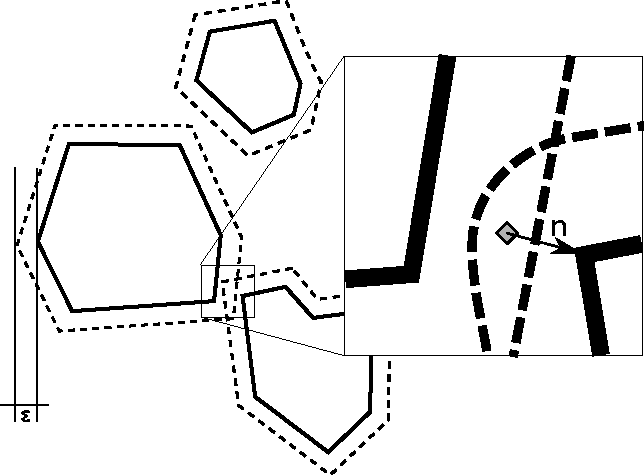
\includegraphics[width=0.45\textwidth]{sketches/minkowski.pdf}
  \end{center}
  \caption{
    Left: Three particles with their $\epsilon $ environment. The particles do
    not penetrate each other, but two particles plus their $\epsilon $
    environment penetrate and create one contact point with a normal. 
  }
  \label{figure:minkowski}
\end{figure}

As we apply a solid particle model, contact always is a unique point. 
We define it to be the centre of an overlap region (Figure \ref{figure:minkowski}), i.e.~the
distance $d$ between a particle $A$ and its contact point with a second particle
is $0 < d \leq \epsilon$.
Each contact point is equipped with a normal $n$ pointing from the contact point
to the surface of the contacting body's surface.
As the distance is positive, the normal is well-defined and we have $|n| \leq
\epsilon $.
Please note that the normal direction depends on whether we make particle $A$
being hit by particle $B$ or the other way round: each normal associated with a
particle points along the outer normal of the body.
Despite the fact that we employ a rigid body model, multiple contact points
between two bodies may exist as particles may be concave and their Minkowsi sum
may overlap.


For two given particles $A$ and $B$ with corresponding sets of triangles
$\mathbb{T}_A$ and $\mathbb{T}_B$, the contact detection thus reads:
Loop over all triangle pairs $t_i \in \mathbb{T}_A, t_j \in \mathbb{T}_B$ and
identify those pairs that are closer than $2\epsilon $.
For those close, determine the middle point along the closest distance. 
The point equals the contact points while the distance vector identifies
its normal.
Add the contact point to a contact point set $\mathbb{C}_A$ and to the set
$\mathbb{C}_B$.
The normal in the latter is inverted.
Such an algorithm has the complexity $\mathcal{O}( | \mathbb{T}_A| \cdot
|\mathbb{T}_B|)$ and makes the overall naive implementation a member of 
$\mathcal{O}( | \mathbb{T} |_{max}^2  )$ if $| \mathbb{T} |_{max} )$
is the maximum number of triangles per particle.


{\bf Force model.}
We apply the linear spring-dashpot force model from Cundall and
Strack \cite{19,Samiei} to study the efficiency of our implementation.
Per particle $A$, it accumulates all contact points in $\mathbb{C}_A$ into one
translational and one rotational repulsive force with some damping.
We make $\mathbb{C}_A$ subject to a postprocessing which eliminates all
collision point duplicates which is all duplicates that are closer than
$min(h_{A,min},h_{B,min})$. 
It is the smallest face length of the meshes representing $A$ and $B$.
No contact point may be closer than this value.
On the preprocessed contact point set $\mathbb{C}_A$ we then determine
\begin{eqnarray}
%   f_{trans} = \sum _{c \in \mathbb{C}_A} 
%   -k_{repulsive} (\epsilon - |n|) \frac{n}{|n|}
%   \\
  f_{trans} = \sum _{c \in \mathbb{C}_A} 
  \min \left( 0, -k_{repulsive} (\epsilon - |n|) + k_{damp}
  \frac{(v_B-v_A,n)}{|n|}  \right) \frac{n}{|n|}
  \label{equation:forces:translational}
  \\
  f_{rot} = \sum _{c \in \mathbb{C}_A}
  \label{equation:forces:rotational}
\end{eqnarray}

%What are the expensive phases 
\noindent
$k_{repulsive}$ and $k_{damp}$ are material coefficients. 
We use the normal's norm to determine the model's penetration depth, while the
change rate of this depth is derives from the projection of the relative
velocity between the two particles onto the normal vector.
We use the the particles' velocities $v_A$ and $v_B$ here.
The $\min $ function ensures that the force always pulls particle away from each
other. 
There is no particle attraction.


Our Newtonian DEM code relies solely on pair-wise interactions so far. 
With a modifcation of
($\ref{equation:forces:rotational}$,$\ref{equation:forces:rotational}$), it is
however possible to introduce more sophisticated force patterns.
We note that the complexity of the force computation depends solely on the size
of $\mathbb{C}$ if we anticipate that we have to run over all particles to
update their position in space due to momentum anyway.
$\mathbb{C}$ typically is very small if particles are of reasonably the same
size. 
If particle sizes vary dramatically, comparably large particles experience
contact forces from many small particles.
In this case, there are however few large particles compared to the overall
number of particles.


{\bf Time stepping.}
For the present work, we rely on an explicit Euler as simplest time stepping
scheme possible.
We implement a symplectic scheme where the velocity is updated with the forces
before the position is updated with the new velocity \cite{Samiei,37}. 
While the extension to implicit schemes is beyond scope \cite{xxx}, our outlook
does discuss more sophisticated and adaptive time step choices which translate
the present time-driven scheme into an event-driven algorithm \cite{xxx}.


\section{Algorithm outline}
\label{section:algorithm}
 
\begin{algorithm}
 
   Blueprint of explicit DEM code's overall structure.
 
 \label{algorithm:dem-blueprint}
% \SetAlgoNoLine
 \begin{algorithmic}[1]
   \For{$t < T$}
   
	\For{i = 0 to N triangles}

		\For {j = i+1 to N triangles}
				
			\State $distance = TTD(i,j)$
				
			\If{(distance $<$ margin) AND ParticleID(i) != ParticleID(j)}

				\State $contact(PID(i)).add(point, normal)$

			\EndIf
			
		\EndFor
			
	\EndFor


	\For{z = 0 to NB particles}

		\For {k = 0 to contacts(z).size()}

			\State $force = granular(velocity(z), position(z), contacts(z).getcontact(k))$

		\EndFor
	
	\EndFor    
    
     \State $t \gets t + \Delta t$
   \EndFor   

 \end{algorithmic}
\end{algorithm} 


We focus on DEM with explicit time stepping (Algorithm \ref{algorithm:dem-blueprint}). 
A straightforward implementation consists of one outer time stepping loop
hosting three inner loops. 
The first inner loop detects contact points between particles' triangles and
check each triangle vs.~the others.
It thus has to loop over the particles.
The second loop runs over these contact points and translates them into forces.
While contact points could in principle be translated into forces straightaway,
it makes sense to outsource the force computation into a separate algorithm
phase.
The third loop applies the forces to the particles and updates the particle
positions.
It has to loop over all particles.


{\bf Contact detection.}
We employ a visco-elastic particle model with spring forces here, where the
actual particle is incompressible.
However, it is equipped with a small halo layer of size $\epsilon >0$:
While the particles are rigid bodies, two particles are assumed to contact each
other if their distance is smaller than $2\epsilon$. 
However, the distance always is positive.
Such an approach equals a Minkowsi sum approach where the actual particles are
blown up by a circle with radius $\epsilon$ and may penetrate each other up to
depth of $\epsilon $.


\begin{figure}[htb]
  \begin{center}
    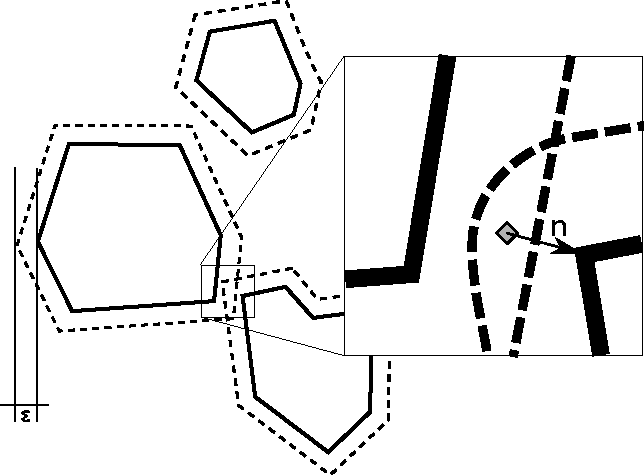
\includegraphics[width=0.45\textwidth]{sketches/minkowski.pdf}
  \end{center}
  \caption{
    Left: Three particles with their $\epsilon $ environment. The particles do
    not penetrate each other, but two particles plus their $\epsilon $
    environment penetrate and create one contact point with a normal. 
  }
  \label{figure:minkowski}
\end{figure}

As we apply a solid particle model, contact always is a unique point. 
We define it to be the centre of an overlap region (Figure \ref{figure:minkowski}), i.e.~the
distance $d$ between a particle $A$ and its contact point with a second particle
is $0 < d \leq \epsilon$.
Each contact point is equipped with a normal $n$ pointing from the contact point
to the surface of the contacting body's surface.
As the distance is positive, the normal is well-defined and we have $|n| \leq
\epsilon $.
Please note that the normal direction depends on whether we make particle $A$
being hit by particle $B$ or the other way round: each normal associated with a
particle points along the outer normal of the body.
Despite the fact that we employ a rigid body model, multiple contact points
between two bodies may exist as particles may be concave and their Minkowsi sum
may overlap.


For two given particles $A$ and $B$ with corresponding sets of triangles
$\mathbb{T}_A$ and $\mathbb{T}_B$, the contact detection thus reads:
Loop over all triangle pairs $t_i \in \mathbb{T}_A, t_j \in \mathbb{T}_B$ and
identify those pairs that are closer than $2\epsilon $.
For those close, determine the middle point along the closest distance. 
The point equals the contact points while the distance vector identifies
its normal.
Add the contact point to a contact point set $\mathbb{C}_A$ and to the set
$\mathbb{C}_B$.
The normal in the latter is inverted.
Such an algorithm has the complexity $\mathcal{O}( | \mathbb{T}_A| \cdot
|\mathbb{T}_B|)$ and makes the overall naive implementation a member of 
$\mathcal{O}( | \mathbb{T} |_{max}^2  )$ if $| \mathbb{T} |_{max} )$
is the maximum number of triangles per particle.


{\bf Force model.}
We apply the linear spring-dashpot force model from Cundall and
Strack \cite{19,Samiei} to study the efficiency of our implementation.
Per particle $A$, it accumulates all contact points in $\mathbb{C}_A$ into one
translational and one rotational repulsive force with some damping.
We make $\mathbb{C}_A$ subject to a postprocessing which eliminates all
collision point duplicates which is all duplicates that are closer than
$min(h_{A,min},h_{B,min})$. 
It is the smallest face length of the meshes representing $A$ and $B$.
No contact point may be closer than this value.
On the preprocessed contact point set $\mathbb{C}_A$ we then determine
\begin{eqnarray}
%   f_{trans} = \sum _{c \in \mathbb{C}_A} 
%   -k_{repulsive} (\epsilon - |n|) \frac{n}{|n|}
%   \\
  f_{trans} = \sum _{c \in \mathbb{C}_A} 
  \min \left( 0, -k_{repulsive} (\epsilon - |n|) + k_{damp}
  \frac{(v_B-v_A,n)}{|n|}  \right) \frac{n}{|n|}
  \label{equation:forces:translational}
  \\
  f_{rot} = \sum _{c \in \mathbb{C}_A}
  \label{equation:forces:rotational}
\end{eqnarray}

%What are the expensive phases 
\noindent
$k_{repulsive}$ and $k_{damp}$ are material coefficients. 
We use the normal's norm to determine the model's penetration depth, while the
change rate of this depth is derives from the projection of the relative
velocity between the two particles onto the normal vector.
We use the the particles' velocities $v_A$ and $v_B$ here.
The $\min $ function ensures that the force always pulls particle away from each
other. 
There is no particle attraction.


Our Newtonian DEM code relies solely on pair-wise interactions so far. 
With a modifcation of
($\ref{equation:forces:rotational}$,$\ref{equation:forces:rotational}$), it is
however possible to introduce more sophisticated force patterns.
We note that the complexity of the force computation depends solely on the size
of $\mathbb{C}$ if we anticipate that we have to run over all particles to
update their position in space due to momentum anyway.
$\mathbb{C}$ typically is very small if particles are of reasonably the same
size. 
If particle sizes vary dramatically, comparably large particles experience
contact forces from many small particles.
In this case, there are however few large particles compared to the overall
number of particles.


{\bf Time stepping.}
For the present work, we rely on an explicit Euler as simplest time stepping
scheme possible.
We implement a symplectic scheme where the velocity is updated with the forces
before the position is updated with the new velocity \cite{Samiei,37}. 
While the extension to implicit schemes is beyond scope \cite{xxx}, our outlook
does discuss more sophisticated and adaptive time step choices which translate
the present time-driven scheme into an event-driven algorithm \cite{xxx}.


\section{Algorithm outline}
\label{section:algorithm}
 
\begin{algorithm}
 
   Blueprint of explicit DEM code's overall structure.
 
 \label{algorithm:dem-blueprint}
% \SetAlgoNoLine
 \begin{algorithmic}[1]
   \For{$t < T$}
   
	\For{i = 0 to N triangles}

		\For {j = i+1 to N triangles}
				
			\State $distance = TTD(i,j)$
				
			\If{(distance $<$ margin) AND ParticleID(i) != ParticleID(j)}

				\State $contact(PID(i)).add(point, normal)$

			\EndIf
			
		\EndFor
			
	\EndFor


	\For{z = 0 to NB particles}

		\For {k = 0 to contacts(z).size()}

			\State $force = granular(velocity(z), position(z), contacts(z).getcontact(k))$

		\EndFor
	
	\EndFor    
    
     \State $t \gets t + \Delta t$
   \EndFor   

 \end{algorithmic}
\end{algorithm} 


We focus on DEM with explicit time stepping (Algorithm \ref{algorithm:dem-blueprint}). 
A straightforward implementation consists of one outer time stepping loop
hosting three inner loops. 
The first inner loop detects contact points between particles' triangles and
check each triangle vs.~the others.
It thus has to loop over the particles.
The second loop runs over these contact points and translates them into forces.
While contact points could in principle be translated into forces straightaway,
it makes sense to outsource the force computation into a separate algorithm
phase.
The third loop applies the forces to the particles and updates the particle
positions.
It has to loop over all particles.


{\bf Contact detection.}
We employ a visco-elastic particle model with spring forces here, where the
actual particle is incompressible.
However, it is equipped with a small halo layer of size $\epsilon >0$:
While the particles are rigid bodies, two particles are assumed to contact each
other if their distance is smaller than $2\epsilon$. 
However, the distance always is positive.
Such an approach equals a Minkowsi sum approach where the actual particles are
blown up by a circle with radius $\epsilon$ and may penetrate each other up to
depth of $\epsilon $.


\begin{figure}[htb]
  \begin{center}
    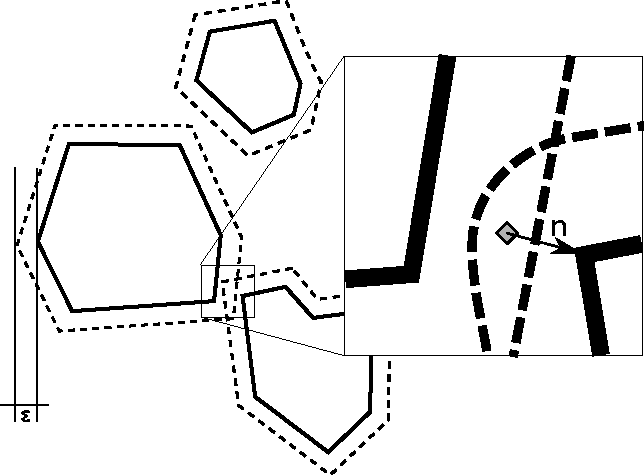
\includegraphics[width=0.45\textwidth]{sketches/minkowski.pdf}
  \end{center}
  \caption{
    Left: Three particles with their $\epsilon $ environment. The particles do
    not penetrate each other, but two particles plus their $\epsilon $
    environment penetrate and create one contact point with a normal. 
  }
  \label{figure:minkowski}
\end{figure}

As we apply a solid particle model, contact always is a unique point. 
We define it to be the centre of an overlap region (Figure \ref{figure:minkowski}), i.e.~the
distance $d$ between a particle $A$ and its contact point with a second particle
is $0 < d \leq \epsilon$.
Each contact point is equipped with a normal $n$ pointing from the contact point
to the surface of the contacting body's surface.
As the distance is positive, the normal is well-defined and we have $|n| \leq
\epsilon $.
Please note that the normal direction depends on whether we make particle $A$
being hit by particle $B$ or the other way round: each normal associated with a
particle points along the outer normal of the body.
Despite the fact that we employ a rigid body model, multiple contact points
between two bodies may exist as particles may be concave and their Minkowsi sum
may overlap.


For two given particles $A$ and $B$ with corresponding sets of triangles
$\mathbb{T}_A$ and $\mathbb{T}_B$, the contact detection thus reads:
Loop over all triangle pairs $t_i \in \mathbb{T}_A, t_j \in \mathbb{T}_B$ and
identify those pairs that are closer than $2\epsilon $.
For those close, determine the middle point along the closest distance. 
The point equals the contact points while the distance vector identifies
its normal.
Add the contact point to a contact point set $\mathbb{C}_A$ and to the set
$\mathbb{C}_B$.
The normal in the latter is inverted.
Such an algorithm has the complexity $\mathcal{O}( | \mathbb{T}_A| \cdot
|\mathbb{T}_B|)$ and makes the overall naive implementation a member of 
$\mathcal{O}( | \mathbb{T} |_{max}^2  )$ if $| \mathbb{T} |_{max} )$
is the maximum number of triangles per particle.


{\bf Force model.}
We apply the linear spring-dashpot force model from Cundall and
Strack \cite{19,Samiei} to study the efficiency of our implementation.
Per particle $A$, it accumulates all contact points in $\mathbb{C}_A$ into one
translational and one rotational repulsive force with some damping.
We make $\mathbb{C}_A$ subject to a postprocessing which eliminates all
collision point duplicates which is all duplicates that are closer than
$min(h_{A,min},h_{B,min})$. 
It is the smallest face length of the meshes representing $A$ and $B$.
No contact point may be closer than this value.
On the preprocessed contact point set $\mathbb{C}_A$ we then determine
\begin{eqnarray}
%   f_{trans} = \sum _{c \in \mathbb{C}_A} 
%   -k_{repulsive} (\epsilon - |n|) \frac{n}{|n|}
%   \\
  f_{trans} = \sum _{c \in \mathbb{C}_A} 
  \min \left( 0, -k_{repulsive} (\epsilon - |n|) + k_{damp}
  \frac{(v_B-v_A,n)}{|n|}  \right) \frac{n}{|n|}
  \label{equation:forces:translational}
  \\
  f_{rot} = \sum _{c \in \mathbb{C}_A}
  \label{equation:forces:rotational}
\end{eqnarray}

%What are the expensive phases 
\noindent
$k_{repulsive}$ and $k_{damp}$ are material coefficients. 
We use the normal's norm to determine the model's penetration depth, while the
change rate of this depth is derives from the projection of the relative
velocity between the two particles onto the normal vector.
We use the the particles' velocities $v_A$ and $v_B$ here.
The $\min $ function ensures that the force always pulls particle away from each
other. 
There is no particle attraction.


Our Newtonian DEM code relies solely on pair-wise interactions so far. 
With a modifcation of
($\ref{equation:forces:rotational}$,$\ref{equation:forces:rotational}$), it is
however possible to introduce more sophisticated force patterns.
We note that the complexity of the force computation depends solely on the size
of $\mathbb{C}$ if we anticipate that we have to run over all particles to
update their position in space due to momentum anyway.
$\mathbb{C}$ typically is very small if particles are of reasonably the same
size. 
If particle sizes vary dramatically, comparably large particles experience
contact forces from many small particles.
In this case, there are however few large particles compared to the overall
number of particles.


{\bf Time stepping.}
For the present work, we rely on an explicit Euler as simplest time stepping
scheme possible.
We implement a symplectic scheme where the velocity is updated with the forces
before the position is updated with the new velocity \cite{Samiei,37}. 
While the extension to implicit schemes is beyond scope \cite{xxx}, our outlook
does discuss more sophisticated and adaptive time step choices which translate
the present time-driven scheme into an event-driven algorithm \cite{xxx}.


\section{Grid meta data structures}
\label{section:grid}

Various speedup techniques such as linked-cell lists \cite{xxx} and Verlet lists
\cite{xxxx} reduce the quadratic complexity in DEM codes.
Notably inspiration in this context stems from the molecular dynamics community
\cite{mattutis:24,wolfgang}. 
In the present paper, we propose to rely on a generalised tree-based linked-cell
technique that allows us to efficiently treat particles of a vast range of diameters.
Three observations support this design decision:
First, particles colliding with other particles are close to these particles.
It thus is sufficient to scan a certain environment around each particle for
potential collision partners.
We do not have to run through all particles per particle.
We thus split up the domain into control volumes.
They are cubic as this simplifies the implementation compared to control volumes
of more flexible shapes.
Second, we may choose these control volumes to be larger than the biggest
particle diameter. 
For a particle held in a particular control volume (cell), it is thus sufficient
to check the $3^d-1$ neighbouring cells whether they host other particles that
might collide. 
$d$ is the spatial dimension.
Third, the previous decision is problematic if the particles are of extremely
different size. 
The cell size is determined by the largest particle diameter. 
If we use a uniform cell size, many uneccessary collision checks are performed
for small particles.
If we use an adaptive grid, it is tricky to design the grid such that only
direct neighbouring cells have to be studied.
We thus, third, observe that a cascade of grids might be useful: If we have
several grids embedded into each other, we can store each particle in the grid
suiting its diameter.
Particles of one grid then have to be checked agains particles in their
neighbouring cell as well as neighbouring cells on coarser grid resolution
levels.
There is no need to check a particle of one grid resolution with particles of a
finer grid resolution---if a particle $A$ collides with a particle $B$, particle
$B$ also collides with particle $A$ and such relations thus are already
detected.


Alternative approaches select the mesh size to accomodate the minimal particle
diameter \cite{mattutis}.
In this case, larger particles overlap multiple cells.
Such an approach requires more sophisticated bookkeeping of particle-cell
relations. 
The idea is not followed up here.
Instead, we prioritise algorithm simplicity---a property that is notably enabled
through trees decomposing the computational domain.


A spacetree is a space-partitioning data structure constructed recursively.
The computational domain is embedded into a unit cube.
We cut the unit cube into three equidistant pieces along each coordinate axis. 
This yields 27 new cubes. 
They are called children of the bounding box cube which is the root.
For each of the children, we continue recursively to evaluate the split
decision. 
The decision to cut into three parts results from the fact that we rely on a
code base based upon three-partitioning \cite{Software:Peano}.
Bipartitioning, i.e.~the classic octree, works as well.


The construction scheme yields a cascade of ragged regular Cartesian grids that
are embedded into each other.
Each cell besides the root has a unique parent cell.
While we could make the cells hold particles, we propose to use a
multiscale, vertex-based scheme spanning a dual meta grid
\cite{Weinzierl:16:PIC}.
A vertex is unique through its spatial position plus its level. 
The level is the number of refinement steps required at least to create one of
its adjacent cells.
Each vertex holds a list of particles.
A particles is always stored on the finest grid level where the cells' edge
length is still bigger than its diameter.
A particle is always associated to the vertex next to its geometric centre,
i.e.~any vertex has a list of all particles close to it on the same level.
Links from the vertices to the particles are realised as pointers. 
If a particle moves, we have to update the links, but we do not move
geometric data in memory.


{\bf Grid traversal.}
With a grid at hand, we may map the algorithmic steps from Algorithm
\ref{algorithm:dem-blueprint} onto a grid traversal.
For the traversal, we rely on a combination of a depth-first order with
space-filling curve \cite{Weinzierl:2009:Diss,Weinzierl:11:Peano}.
From a DEM point of view, the exact traversal realisation however is not that
relevant as long as the traversal is a real tree traversal, i.e.~runs through
all levels of the underlying spacetree.

\begin{figure}
  \begin{center}
    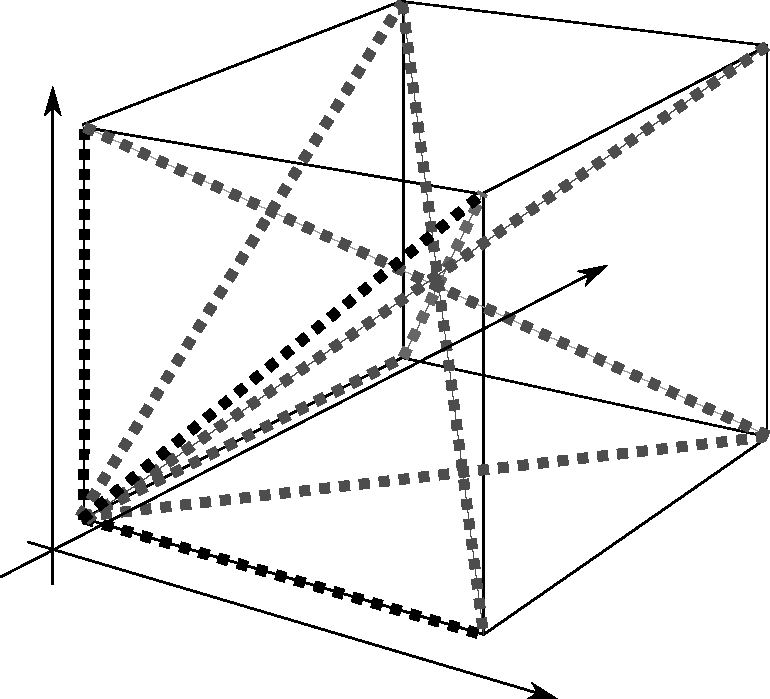
\includegraphics[width=0.25\textwidth]{sketches/collision-cube.pdf}
    \hspace{0.2cm}
    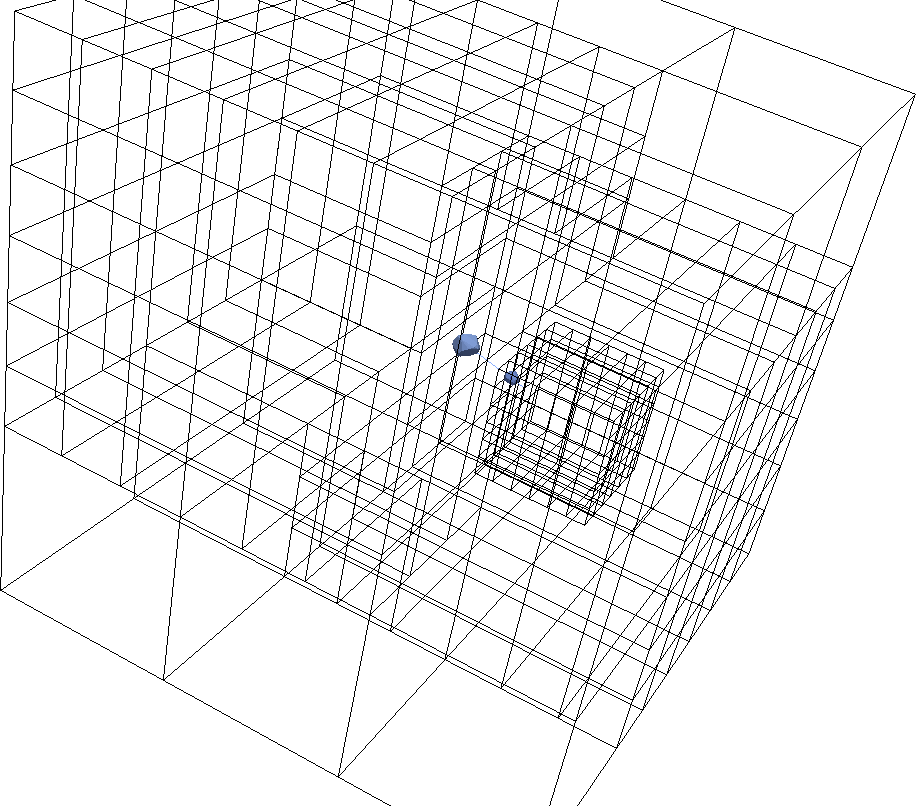
\includegraphics[width=0.3\textwidth]{experiments/two-bodies/visualisation/adaptive-grid01.png}
    \hspace{0.2cm}
    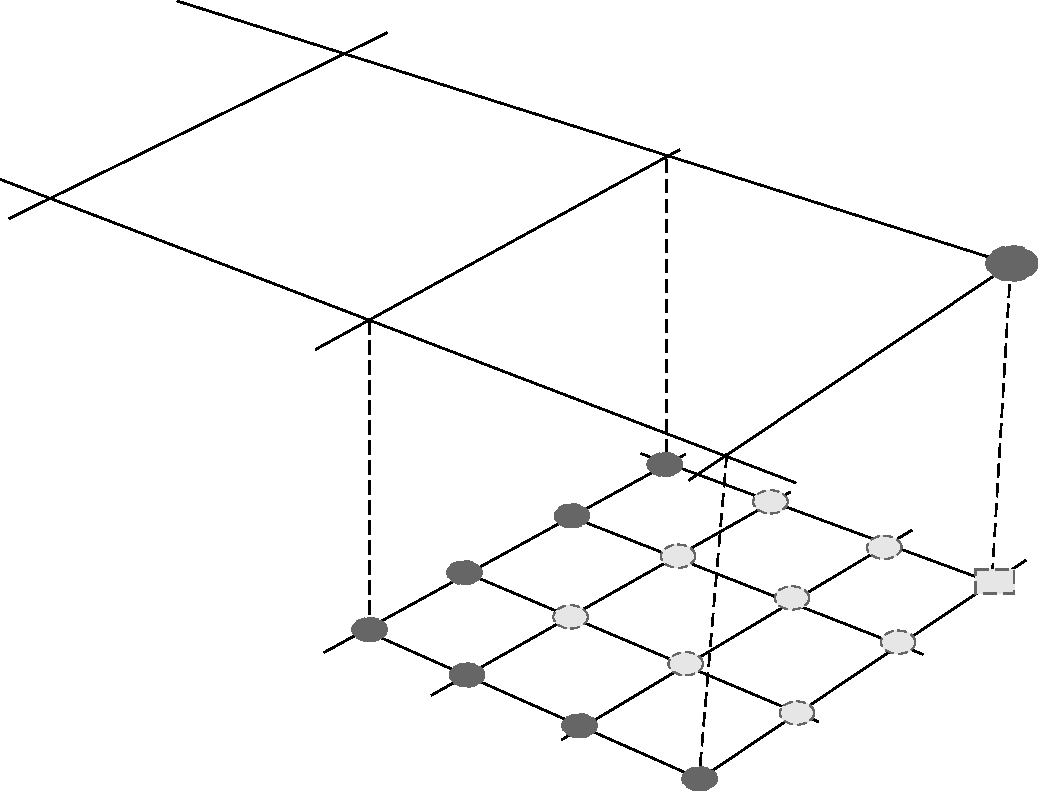
\includegraphics[width=0.3\textwidth]{sketches/multigrid.pdf}
  \end{center}
  \caption{
    Left: Whenever the grid traversal enters a cell, it checks whether particles
    assigned to one vertex do collide with particles assigned to another vertex.
    To avoid redundant collision computations, we check only some vertex pairs
    (dotted, larger lines).
    Middle: Two particles approach each other. As they are of different size,
    they might be held on different spacetree resolution levels.
    Right: In the adaptive case, particles are dropped from the coarse levels
    into the fine grid (rectangular marker) if new grid levels are added. The
    bright round vertices are children of the marked coarse grid vertex. The
    bright and the dark round markers' vertices together are the descendants of
    the marked coarse grid vertex.
  }
  \label{figure:collision-cube}
\end{figure}


We then write down the algorithm as a set of events, i.e.~we specify which
operations are performed if a vertex is read for the very first time \linebreak
(\texttt{touchVertexFirstTime}), if a cell is entered
(\texttt{enterCell}), and so forth.
Besides the actual grid hosting the particles, the grid sweeps build and
maintain two further sets of collision points (Algorithm \ref{algorithm:grid-based-dem}).

\begin{algorithm}
 \caption{A grid-based DEM implementation.}
 \label{algorithm:grid-based-dem}
 \begin{algorithmic}[1]
  \Function{traverseGrid}{$\mathcal{C}$}
   \State $\mathcal{C}_{old} \gets \mathcal{C}$
   \State $\mathcal{C} \gets \emptyset$
   \While{traversal continues}
    \If{\texttt{touchVertexFirstTime}}
     \ForAll{particles $p$ associated to vertex}
      \ForAll{contact points $c \in \mathcal{C}_{old}$ associated to $p$}
       \State Update $f_{trans}(p)$ through $c$
       \State Update $f_{rot}(p)$ through $c$
      \EndFor
     \EndFor
     \ForAll{particles $p$ associated to vertex}
      \State Update particle incl.~its triangles
     \EndFor
     \ForAll{particle pairs $(p_i,p_j)$ associated to vertex}
       \State $\mathcal{C} \gets \mathcal{C} \cup $
       \Call{findCollisions}{$p_i,p_j$}
     \EndFor
    \EndIf
    \If{\texttt{enterCell}}
     \ForAll{$2^d$ vertices adjacent to cell}
      \ForAll{particles $p$ associated to vertex}
       \If{particle should be associated to different vertex}
        \State Reassign particle
       \EndIf
      \EndFor
     \EndFor
     \ForAll{$(p_i,p_j)$ associated to different vertices (cmp.~figure)} 
      \State $\mathcal{C} \gets \mathcal{C} \cup $
       \Call{findCollisions}{$p_i,p_j$}
     \EndFor
    \EndIf
   \EndWhile
  \EndFunction

  \Function{main}{$T$}   
   \State $\mathcal{C} \gets \emptyset $
   \State $t \gets 0 $
   \For{$t < T$}
    \State \Call{traverseGrid}{$\mathcal{C}$}
    \State $t \gets t + \Delta t$
   \EndFor
  \EndFunction
 \end{algorithmic}
\end{algorithm} 


Our grid-based realisation is characterised by few properties:
\begin{itemize}
  \item When we load a vertex for the very first time, we make all particles
  associated to this vertex move. 
  \item When we load a vertex, we do compare all the particles associated to
  this vertex with each other and identify collision points. The comparison of
  particles associated to different vertices is realised when we enter a cell.
  Here, we do compare the vertex pairs from Figure \ref{figure:collision-cube}---left bottom
  front vertex with right bottom front vertex, all diagonal combinations, and
  so forth---such that we avoid multiple evaluations of vertex pairs. For 
  boundary cells, some special case distinctions yielding additional checks are
  added. If a cell is traversed, we assume that all its adjacent vertices are
  available, i.e.~have been read before.
  \item Whenever we run into a cell, we run through all the adjacent vertices
  and their particles. They all already have an updated position, as any vertex
  has been loaded before and thus been subject to \texttt{touchVertexFirstTime}.
  If a particle is associated to the 'wrong' vertex as it has moved and should 
  be assigned to another vertex of the cell, we do the reassignment. A particle
  may move at most one cell of its corresponding level a time.
  \item The vertex comparisons yield a set of collision points. This set is kept
  persistent for the subsequent traversal: one time step of the scheme is
  realised per two grid traversal. The amortised cost however still is one time
  step per grid traversal. This scheme picks up the idea of pipelining
  \cite{xxx,xxx,xxx}. Collision data is mapped onto the particles when we read a
  particle for the first time in the subsequent traversal. Immediately after the
  forces acting on a particle are determined, we do update the particle's
  property and also update the geometric data due to translation and rotation.
\end{itemize}

\noindent
The extension of the present scheme to multiscale trees is detailed below.
To make the algorithm correct, each contact point set between two particles does
exist twice with inverse normals.
Each set furthermore is augmented with a copy of the corresponing partner
particles' global data (mass, velocity, momentum).
Otherwise, we would have to search for this data and build up global indices,
and have to be aware that the particle's data already might have been subject to
the next time step.


\begin{observation}
The algorithm realises a single-pass policy. Geometric data is written only once
per traversal, and is read only when we read in a vertex for the first time and
when we run through a cell.
The implementation's pressure on the memory subsystem thus is minimalistic as
long as the spatial and temporal grid access locality \cite{dime} is high which
yields high cache hit rates.
We rely on a space-filling curve to
run through the grid \cite{Weinzierl:2009:Diss,Weinzierl:11:Peano} and thus
guarantee such a two-fold locality.
\end{observation}


\noindent
More sophisticated explicit schemes can be realised with the same single-touch
policy if we hold additional data per particle (acceleration, e.g.).
Such an approach picks up ideas of pipelining \cite{xxx}.
The GEAR algorithm \cite{33,34} is an example for such a scheme.
However, the class of predicator-corrector schemes fits if and only if we shift
them by half a grid traversal, i.e.~perform the prediction right after a
corrector in the same traversal.
We introduce such a shift for equation system solvers in \cite{Reps} and extend
them to hyperbolic equation system solvers in \cite{Charrier}.




{\bf Regular grid.}
The spacetree formalism allows us to realise at least three grid variants. 
A very simple refines all spacetree nodes all the time as long as the resulting
cell mesh size is bigger than the largest particle diameter.
Such a strategy yields a regular Cartesian grid. 

{\bf Dynamically adaptive grid.}
Our dynamically adaptive grid is characterised by two ingredients: mesh
refinement control and inter-grid particle treatment.
In \texttt{touchVertexFirstTime}, our code analyses what the smallest diameter
of all the particles held by the vertex is.
If this diameter is smaller than $1/3$ of the mesh width corresponding to the
vertex's level, then the region around the vertex is refined.
If we run into a vertex, we check whether there are any spatially coinciding
vertices in the tree on a coarser level.
If such vertices do exist, we run through all of their particles and move them
one level down if the diameter permits.
The scheme successively drops the particles down the grid hierarchies.

\begin{figure}
 \begin{center}
  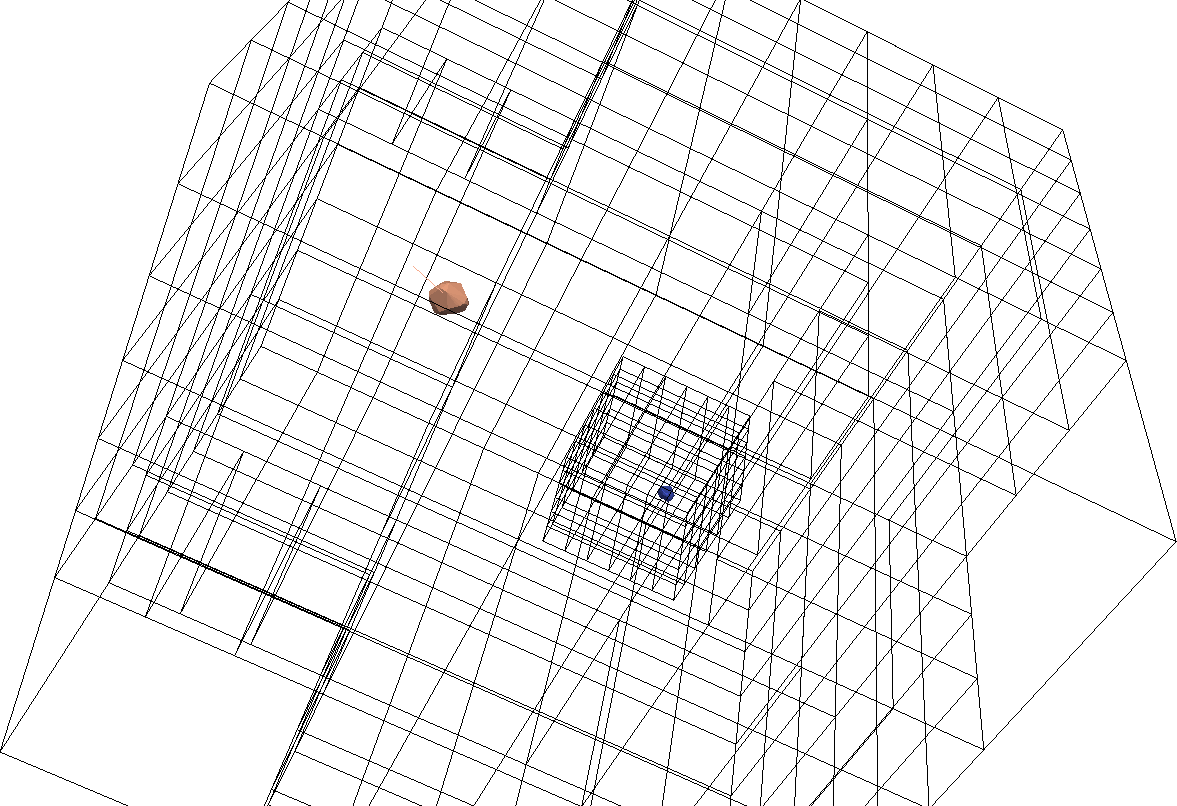
\includegraphics[width=0.4\textwidth]{experiments/two-bodies/visualisation/adaptive-grid00.png}
  \hspace{1.1cm}
  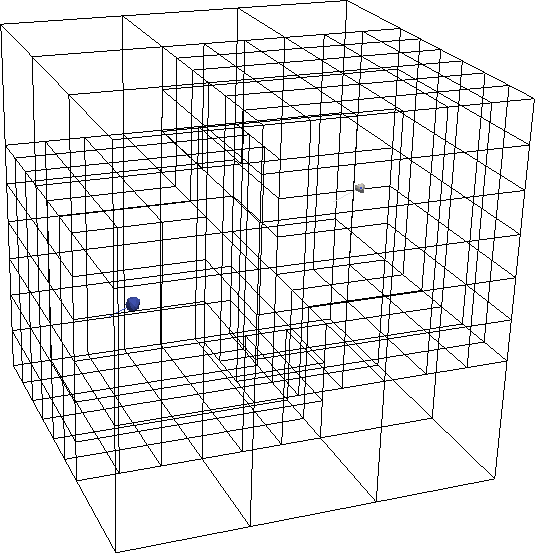
\includegraphics[width=0.25\textwidth]{experiments/two-bodies/visualisation/reluctant-adaptive-grid00.png}
  \\
  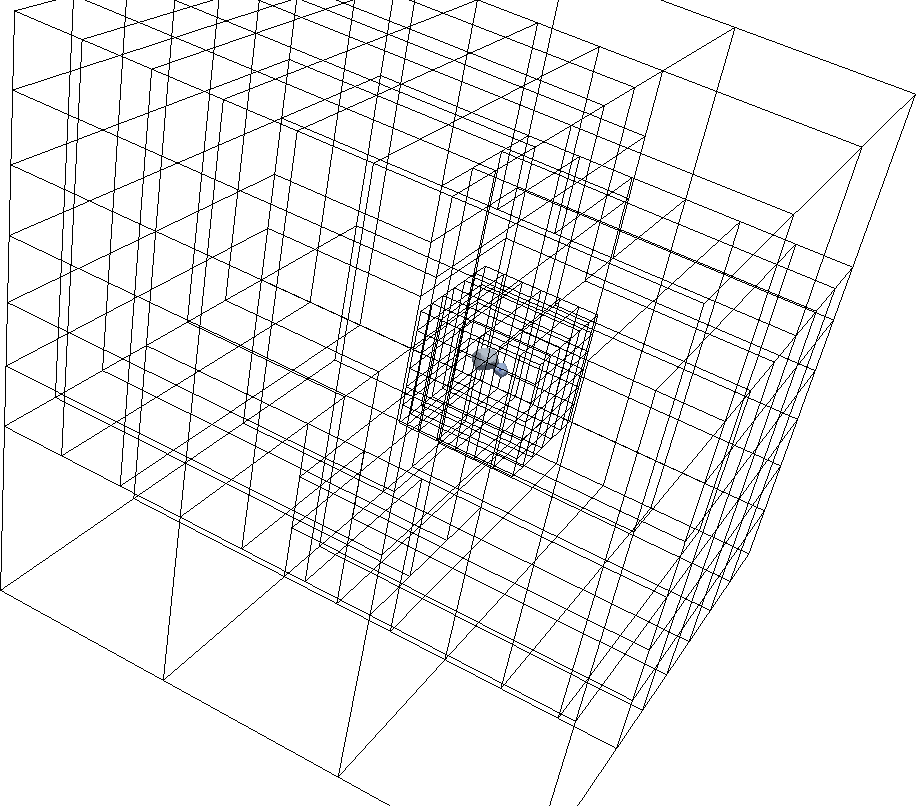
\includegraphics[width=0.3\textwidth]{experiments/two-bodies/visualisation/adaptive-grid02.png}
  \hspace{1.1cm}
  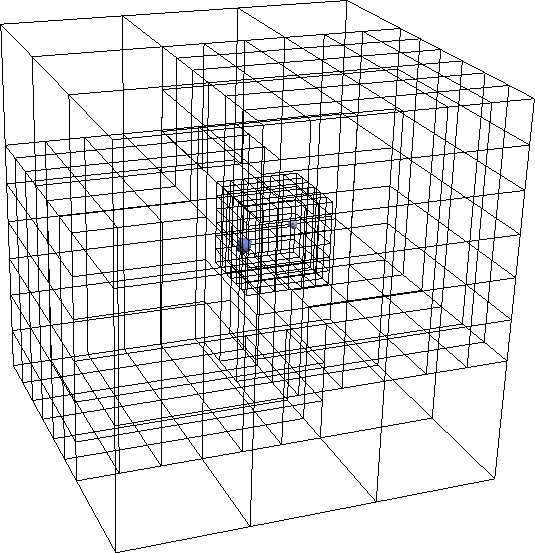
\includegraphics[width=0.3\textwidth]{experiments/two-bodies/visualisation/reluctant-adaptive-grid02.png}
% 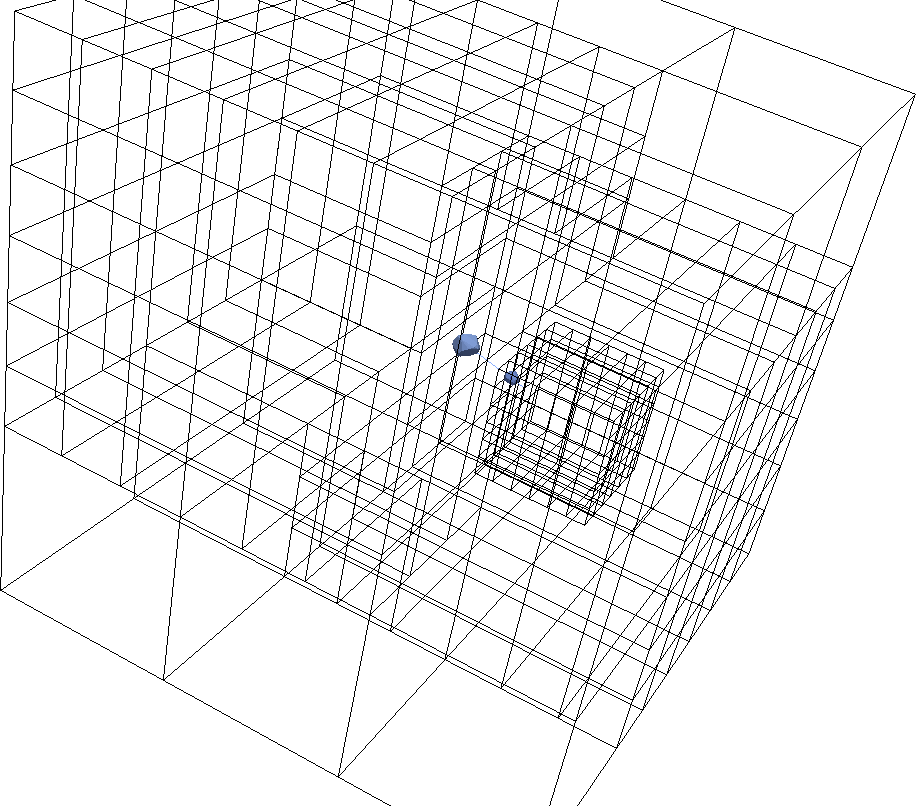
\includegraphics[width=0.3\textwidth]{experiments/two-bodies/visualisation/adaptive-grid01.png}
%   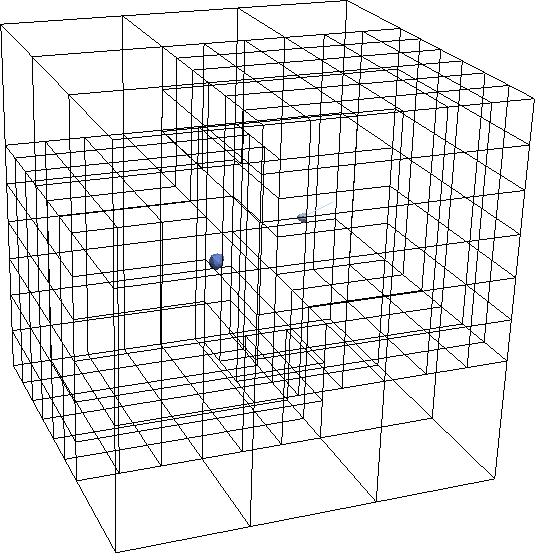
\includegraphics[width=0.3\textwidth]{experiments/two-bodies/visualisation/reluctant-adaptive-grid01.png}\\
%   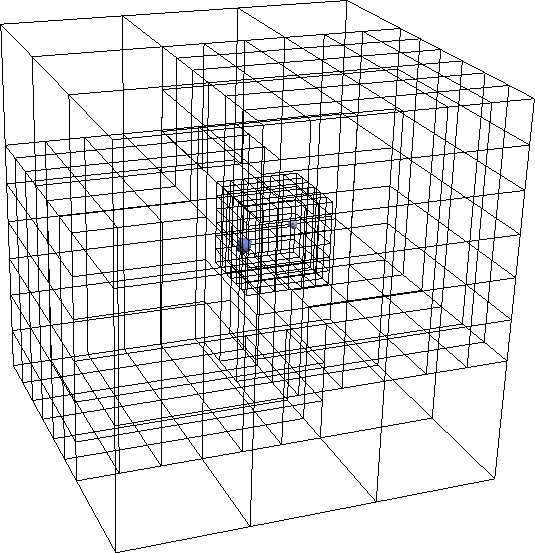
\includegraphics[width=0.3\textwidth]{experiments/two-bodies/visualisation/reluctant-adaptive-grid02.png}
%   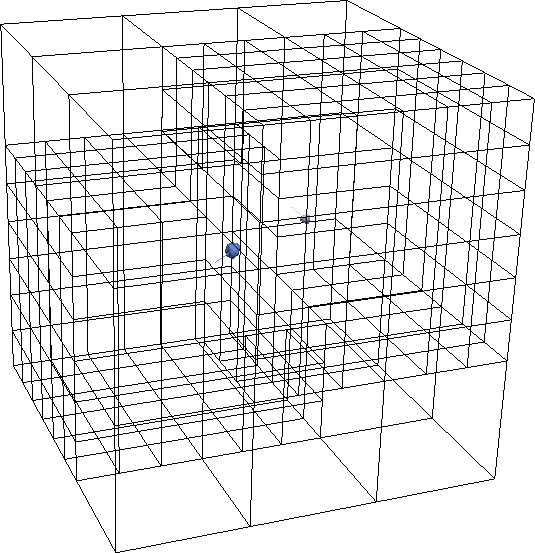
\includegraphics[width=0.3\textwidth]{experiments/two-bodies/visualisation/reluctant-adaptive-grid03.png}\\
 \end{center}
 \caption{
   Two particles crash into each other.
   The adaptive grid refining around each particle while its diameter
   constrains the mesh size (left column).
   The reluctant adaptive grid works with a coarser resolution as long
   as particles are far away from each other (right column).
   Just before they collide, the grid is refined and particles are dropped down
   the resolution levels.
 }
 \label{figure:adaptive-vs-reluctant-grid}
\end{figure}


We define two multiscale relationships between vertices (Figure
\ref{figure:collision-cube}).
A vertex $a$ is a child of a vertex $b$ if all adjacent cells of $a$ are
children of adjacent cells of $b$.
$b$ is the parent vertex of $a$.
A vertex $a$ is a descendant of $b$ if at least one adjacent cell of $a$ is a
child of an adjacent cell of $b$.
$b$ is an ancestor of $a$.
If we delete a vertex $a$ that holds particles, its particles are moved to the
next coarser level and assigned there to the nearest parent of $a$.
Each vertex holds a boolean marker that is set $\bot $ before the vertex is
read for the first time.
If a vertex holds a particle, all the markers of the vertices where it is a
descendent from are set to $\top$.
If a vertex whose adjacent cells all are refined holds $\bot$ at the end of the
multiscale traversal, we coarsen these refined adjacent cells.
We rely on a top-down tree traversal.
The refinement/coarsening procedure then can be evaluated on-the-fly.
It equals an analysed tree grammar \cite{knuth}.

For the multiscale contact detection, we extend the list of particles associated
to a vertex. 
There is the list of actually held particles and a list of virtual particles. 
We run through the grid top down, i.e.~a vertex always is read for the first
time before any of its descendants, and clear virtual particle list first.
Then, we add all particles held in the particle or the virtual particle lists of
any ancestor to the local virtual list.
If we compare all particles with each other that are held by the same vertex, we
do compare the actual particles with all other real particles as well as all
virtual particles.


{\bf A reluctant adaptive grid.}
The dynamically adaptive grid refines rather aggressive: Particles are always
dropped to their corresponing refinement level immediately. 
Fine grid regions thus follow `their' particles (Figure
\ref{figure:adaptive-vs-reluctant-grid}).
This might introduce finer grids than actually required for contact detection
which is an overhead.
Given the one-cell-per-time-step constraint on the particle velocity, we also
restrict the maximum velocity or time step rigorously.
For the present work, this does not have a major impact as we apply uniform
small time step sizes globally. 
For schemes with local time stepping, it however is important, besides overhead
discussions, to keep the grid as coarse as possible as this facilitates big
time step sizes.


Our reluctant adaptive grid works with coarser adaptive grids than the plain
variant through two modifications of the refinement procedure: 
On the one hand, we refine the region around a vertex if the previous criterion
holds and the vertex holds at least two particles.
If only one particle is holds, we stick locally to the grid no matter what the
particular diameter is.
Throughout the inter-vertex contact detection in \texttt{enterCell}, we further
bookkeep the minimum diameter of all the particles involved. 
If this minimal diameter is smaller than the cell, we do refine this cell, too.



\section{Particle storage and vectorisation}
\label{section:vectorisation}

There are three different types of data sets in our minimalistic DEM codes: 
geometric data, behavioural data and meta data. 
Behavioural data is collision data.
It is modelled as struct with location and a normal vector.
Sets $\mathbb{C}$ of collision points are modelled as (dynamic) array of structs
(AoS) augmented with a copy of the collision partner as detailed before.
Spacetrees are our meta data.
The geometry data finally determines how straightforward and fast the collision
detection is. Collision detection is the computationally heavy activity in the
algorithm.
While other DEM discussions speak of a computational phase \cite{xxxx}, we
prefer activity, as the collision detections are split among the grid traversal
and interwoven with other activities.

\begin{figure}
 \begin{center}
  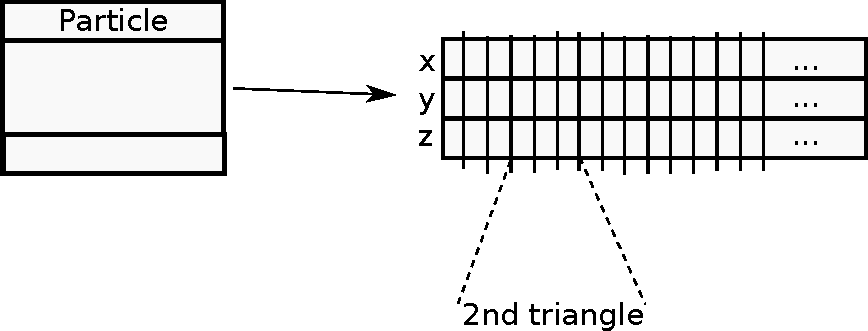
\includegraphics[width=0.5\textwidth]{sketches/data-structure.pdf}
 \end{center}
 \caption{
   Right: The two layer data layout of our DEM code with an AoS on the particle
   level but SoA for the vector entries with replicated vector entries.
 }
 \label{figure:data-structure}
\end{figure}

We propose to realise the geometric data in two layers (Figure
\ref{figure:data-structure}).
A hull struct holds all particle properties such as velocities, rotation, mass,
geometric centre and mass centre.
Vertices refer to these hulls with arrays of structures (AoS).
Hulls link with pointers to the actual geometric data. 
This data is realised as structure of array, i.e.~there is a sequence of
x-coordinates, a sequence of y-coordinates and a sequence of z-coordinates.
These sequences are blown up with redundant data.
The first three entries in the x array hold the x coordinates of the three
vertices of the first triangle of the particle mesh.
The entries four through six hold the coordinates of the second triangle and so
forth. 
The degree of redundancy is determined by the particle mesh.

We accept the increased memory consumption of such a structure but in return are
able to avoid any indirect addressing, process all geometry data in the
collision checks in a stream-like fashion and can align all vector entries. 
SoA data are notouriously difficult to handle if subsets of a dataset are to be
transferred or data is to be reordered.
In our particle handling, a particle is an atomic unity.
It is never teared apart or resorted during the simulation run.
A particle mesh is topologically invariant.

The remainder of this section discusses a function \texttt{findCollisions} that
is passed two particles or two particle meshes respectively and identifies all
contact points. 
Such an operation with quadratic complexity is often wrapped into an additional
check that compares bounding boxes and thus may skip comparisons
\cite{mattutis}.
We abstain from such a check as the spacetree realises a related optimisation.
The following text thus discusses a nested loop with the outer loop
running over all triangles in $\mathbb{T}_A$ and the inner loop running over all
triangles in $\mathbb{T}_B$. 

\subsection{Brute force geometric comparison}

\subsubsection{Segment to Segment Minimum Distance }
The calculation of the distance between segments [8,9] in three dimensions is a geometric calculation that involve getting the closest points by extending the line that they lie on until intersection, if the two lines intersect then the closest point on the two segments is on the boundaries of the segment.
The segment 
$$S1 = [P0, P1]$$
can be formulated as 
$$P(s) = P0+s(P1-P0) = P0+su$$
with a constraint on s, $0<=s<=1$. Similarly, the second segment 
$$S2 = [Q0, Q1]$$
is written as $$Q(t) = Q0+t(Q1-Q0) = Q0+tu$$ with constraint $0<=t<=1$. So, for $sC$ and $tC$ being the closest points on the corresponding extended segments lines L1 and L2, then if  both sC and tC are within the boundaries of the segments then the closest points are also the closest points on the respective segments. 
In the case where sC and tC correspond to points on L1 and L2 outside the range of either segment $S1$ and $S2$, then sC and tC do not also define the closest points on the segments $S1$ and $S2$. So it is necessary to determine points that minimize 
\begin{equation}
w(s,t) = P(s) - Q(t)
\end{equation}
over the ranges of the segments using the corresponding constraints. 
The problem can be formulated into a minimization problem where the equation w is the same as minimizing 
$$|w|^2 = w \cdot w= (P0+su-tv) \cdot (Q0+su-tv)$$

which is a quadratic function of s and t. The relation of $|w|^2$ define a parabolic equation over a (s,t)-plane (See Figure \ref{fig9}) with a minimum at $C = (sC, tC)$, it is strictly growing along the (s,t)-plane with starting point from C. But because segments $S1$ and $S2$ are concerned and not their respective extended lines $L1$ and $L2$, the required minimum region is not C but it is located over a subregion G of the (s,t)-plane. The global minimum at C may lie outside of G, however, in these cases, the minimum always occurs on the boundary of G, and in particular, on the part of G's boundary that is visible to C. That is, there is a line from C to the boundary point which is exterior to G, and it can be said that C can "see" points on this visible boundary of G (See Figure \ref{fig9}).

\begin{figure}[!h]
\centering
\includegraphics[width=0.3\textwidth]{sketches/ss_box} \protect\caption{\label{fig9}(s,t) parameter space with G boundary box C for global minimum}
\end{figure} 

Suppose that we want the minimum distance between two finite segments $S1$ and $S2$, then 
$$G=\{ (s,t) \: \| \: 0 \leq s \leq 1, 0 \leq t \leq 1 \} = [0,1]\times[0,1]$$ 
is a unit square in (s,t) space. The four edges of the square are given by point at $s = 0, s = 1, t = 0, t = 1$. If $C = (sC, tC)$ is outside the G area, then it can "see" at most two edges of G. If $sC < 0$, C can see the $s = 0$ edge, if $sC > 1$, C can see the s = 1 edge, and similarly for tC, so in this way there is an enforcement of the required constraints. When C is not in G, at minimum 1 and at maximum 2 of constraints are active, and they determine which edges of G are candidates for a minimum of $|w| ^2$.
 
For each candidate edge, to compute where the minimum that occurs on that edge, either in its interior or at an endpoint, it is possible to solve for the other unknown parameter since at minimum one is to be found (either t or s). So using the derivative of the $|w^2|$ equation it is always possible to solve for the parameter that is in the interior of G. For example when s = 0, $|w|^2 = ((P0-Q0)-tv) \cdot ((P0-Q0)-tv)$. Taking the derivative with $t$ it possible get a minimum when: $0 = \frac{d}{dt}|w|^2 = -2v \cdot ((P0-Q0)-tv)$.
This gives a minimum on an edge at (0, t0) where $t0 = \frac{(v \cdot (P0-Q0))}{(v \cdot v)}$
If $0 <= t0 < 1$, then this would be the minimum of $|w|^2$ on G, and P(0) and Q(t0) are the two closest points of the two segments. But in the case where t0 is outside G, then either (0,0) or (0,1), would be the minimum along that edge (since $s=0$). Using this method it is possible to perform only a couple of checks to find the minimum of w(s,t) that correspond to the minimum distance between the segments.

\subsubsection{Point to Triangle Minimum Distance}
The other calculation required by the naive approach is to perform the check of point to triangle distance[12, 10, 11]. This test complete the brute force approach since it doesn't leave any  space for cases where triangles are in a configuration where a point - triangle plane distance is the shortest distance in the initial triangle pair minimum distance problem. 

To understand the problem of computing the minimum distance between a point P and a triangle T, it is necessary to understand the parameterised coordinate system of triangles. A triangle can be described by its barycentric coordinates in a way that any point on it can be dependent on two parameters, such that 

$$T(s, t) = B + s \cdot E0 + t \cdot E1$$

where $B = point1$, $E0 = point2-point1$, $E1 = P3 - P1$ for 

$$(s,t) \in D = \{(s,t) : s \in [0,1],t \in [0,1],s + t ≤ 1\}$$ 

The minimum distance is computed by determining the values $(s, t) \in D$ in the squared-distance equation $Q(s, t) = |T(s, t) - P|^2$ where $T(s,t)$ correspond to a point on the triangle closest to P. The function is quadratic and can be written as: 
$$Q(s,t)=as^2 +2bst+ct^2 +2ds+2et+f$$

where $a = E0 \cdot E0$, $b = E0 \cdot E1$, $c = E1 \cdot E1$, $d = E0 \cdot (B - P)$, $e = E1 \cdot (B - P)$, and $f = (B - P) \cdot (B - P)$.

Quadratics are classified by the sign of $ac - b^2$ so for function Q, $ac - b2$ = $(E0 \cdot E0)(E1 \cdot E1) - (E0 \cdot E1)^2$ =$|E0 \cdot E1|^2 >0$. The positivity is based on the assumption that the two edges E0, E1 are linearly independent, so their cross product is a nonzero vector. Q is a continuously differentiable and the minimum occurs at an interior point of D where the gradient $Q = 2(as + bt + d, bs + ct + e) = (0, 0)$ or at a point on the boundary of D. The gradient of Q is zero only when 
$$s = (be - cd)/(ac - b^2)$$ and 
$$t = (bd - ae)/(ac - b^2).$$ 
If $(s,t) \in D$, then minimum of Q is found. For example considering that region 0 (See Figure \ref{fig10}) is the domain of Q, so $(s, t) \in D$. If (s, t) is in region 0, then the point on the triangle closest to P is interior to the triangle, not on its edge.

\begin{figure}[!h]
\centering
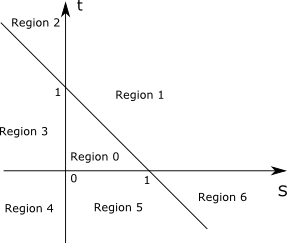
\includegraphics[width=0.4\textwidth]{sketches/pt_regions} \protect\caption{\label{fig10} Regions based on the (s,t) parameters plane}
\end{figure} 

On the other hand if the minimum is not in D then it should be should be on the boundary of the triangle and using the correct active constraints to restrict the solution using the region methodology. So if (s, t) is in region one then the elliptic level curves of Q are those curves in the s,t plane for which Q is constant. 

At the point where Q = (0,0), the level curve degenerates to a single point (s, t). The global minimum of Q occurs there ($V_{min}$). As the level values V increase from $V_{min}$, the corresponding levels are growing away from $(s,t)$. There is a smallest level value V0 for which the corresponding ellipse is tangent to the triangle domain $D$ edge $s+t = 1$ at a value $s = s0 \in [0,1], \: t0 = 1 - s0$. So for any level values $V < V0$, the corresponding ellipses do not intersect $D$. However for any portion of $D$ that intersect elliptic levels V must be $V > V0$. Therefore in this case point $(s0, t0)$ provides the minimum distance between P and the triangle where $t0$ is known $t0 = 1 - s0$ and $s0$ is the only unknown to be solved since the problem is decreased by one dimension. Moreover, when minimization is happening at $\nabla Q(s, 1 − s) = 0$ then there are three cases where $s > 1$ and $s$ has to be restricted to $s=1$ and the minimum occurs at $\nabla Q(1, 0)$ because of the barymetric triangle constraints, similarly if $s < 0$ then minimum occurs when $\nabla Q(0,1)$ or lastly $s \in [0,1]$ and has to be solved for a minimum at $\nabla Q(s,1-s)$.

Similarly the same technique for determining whether the minimum occurs at the endpoints or at the interior interval of the corresponding constraints, is performed for region three and region five (Figure \ref{fig10}). In the case where (s, t) occur in region three then the minimum has to occur at (0, t0) following the process like in region one where $t0 \in [0, 1]$. If $(s, t)$ is located in region five (Figure \ref{fig10}), then the minimum occurs at $(s0, 0)$ where $s0 \in [0, 1]$.  

When $(s, t)$ is located inside region two, there are three possibilities for the elliptic level curve that contact or intersect the boundaries of $D - region0$ area, the contact of the levels with the triangular region may occur in: 
\begin{enumerate}
\item edge where $s + t = 1$ 
\item edge where $s = 0$
\item at point where $t = 0$ and $s = 1$.
\end{enumerate}

That is because although the global minimum occurs in region two, there is a level curve of Q that contact the $D$ but the contact point and the region inside the level curve does not overlap. At these occurrences then the negative of the contacting level curve of Q cannot point inside $D$. For example for region two could be the direction of $-\nabla Q(0,1), -\nabla Q(s,1-t) and -\nabla Q(0,t),$ which points towards the inside of the level curve instead of inside $D$. 

In order to determine which of the three cases occur, it is possible to check which areas are negative so in a way it is possible to eliminate the cases where the contact doesn't occur and where it does. So if $\nabla Q = (Qs, Qt)$ and $Qs$ and $Qt$ are the partial derivatives of Q, it should be the case where $(0, -1) \cdot \nabla Q(0, 1)$ and $(1, -1) \cdot \nabla Q(0, 1)$ are not both  negative. The two vectors $(0, −1)$ and $(1, −1)$ are directions that correspond to the edges $s = 0$ and $s + t = 1$, respectively. The choice of edge $s+t = 1$ or $s = 0$ can be made based on the signs of $(0,-1) \cdot \nabla Q(0,1)$ and $(1, -1) \cdot \nabla Q(0, 1)$. Similarly as for region three, the same calculation technique is used for the regions four and six. 

\clearpage

\begin{algorithm}
 \caption{Brute-force distance calculation.} \label{algorithm:bf}
 \begin{algorithmic}[1]
	\Function{BF}{A, B, C, D, E, F}
	
		\State $T1=[A;B;C;];$
		
		\State $T2=[D;E;F;];$

		\State $list[0]= pt(T2, T1[0]);$

		\State $list[1]= pt(T2, T1[1]);$

		\State $list[2]= pt(T2, T1[2]);$

		\State $list[3]= pt(T1, T2[0]);$

		\State $list[4]= pt(T1, T2[1]);$

		\State $list[5]= pt(T1, T2[2]);$

		\State $ptmin = min(list);$

		\State $list[0]=segseg(T1[0],T1[1],T2(0],T2[1]);$

		\State $list[1]=segseg(T1[0],T1[1],T2[1],T2(2]);$

		\State $list[2]=segseg(T1[0],T1[1],T2[2],T2(0]);$

		\State $list[3]=segseg(T1[1],T1[2],T2[0],T2(1]);$

		\State $list[4]=segseg(T1[1],T1[2],T2[1],T2(2]);$

		\State $list[5]=segseg(T1[1],T1[2],T2[2],T2(0]);$

		\State $list[6]=segseg(T1[2],T1[0],T2[0],T2(1]);$

		\State $list[7]=segseg(T1[2],T1[0],T2[1],T2(2]);$

		\State $list[8]=segseg(T1[2],T1[0],T2[2],T2(0]);$

		\State $ssmin = min(list);$

		\State $min = min(ssmin, ptmin);$

		\State $P = min.p; Q = min.q;$
	\EndFunction
 \end{algorithmic}
\end{algorithm} 


\begin{algorithm}
 \caption{Point to triangle distance algorithm.} \label{algorithm:bf}
 \begin{algorithmic}[1]
	\Function{pt}{T, Point}
		
		%function to evaluate Q(s,t) of triangle T 		
		
		\If{PointProjection in Region 0}
		
			\State {evaluate value of Q}
		
		\EndIf		
		
		\If {PointProjection in Region 1}
		
			\State {determine (s,t) parametric space values}
		
		\EndIf
			
		\If {PointProjection in Region 2}

			\State {determine (s,t) parametric space values}

		\EndIf			
		
		\If {PointProjection in Region 3}
		
			\State {determine (s,t) parametric space values}

		\EndIf
						
		\If {PointProjection in Region 4}
		
			\State {determine (s,t) parametric space values}
		
		\EndIf
				
		\If {PointProjection in Region 5}		

			\State {determine (s,t) parametric space values}

		\EndIf
				
		\If {PointProjection in Region 6}	

			\State {determine (s,t) parametric space values}
			
		\EndIf		
		
		\Return $Q point on triangle$
	\EndFunction
 \end{algorithmic}
\end{algorithm} 

\begin{algorithm}
 \caption{Segment to segment distance algorithm.} \label{algorithm:bf}
 \begin{algorithmic}[1]
	\Function{pt}{segment1, segment2}
		
		%function to evaluate (s,t) of seg1, seg2
		\If {segment1 and segment2 are parallel}		
		
			\Return {any point P on segment1 and any point Q on segment2}
		
		\Else 
			
			\State {Get the closest points sC and tC on the infinite lines L1, L2}
			
			\If {sC < 0, the s = 0 edge is visible}
				
				\State {s = 0}
				
			\EndIf
				
			\If {sC > 0, the s = 1 edge is visible}

				\State {s = 1}			
				
			\EndIf
				
			\If {tC < 0, the t = 0 edge is visible}

				\State {t = 0}

			\EndIf
								
			\If {tC > 0, the t = 1 edge is visible}

				\State { t = 1}

			\EndIf							
		\EndIf
		
		\Return {P, Q points on two segments}
		
	\EndFunction
 \end{algorithmic}
\end{algorithm} 

%
% How does the algorithm work. Robustness
%
Our default brute force approach implementation runs per triangle pair through all possible distance
configurations (Algorithm \ref{algorithm:bf}).
First, we run through all six involved vertices and compute the distance to the
other triangle.
Second, we determine the distances between each line segment-to-line segment combination.
This yields 9+6=15 comparisons in total.
The minimum distance results from a minimum over all computed distances.
It is a robust approach, it always yields the correct answer.


%
% Speed, character
%
The algorithm is \ldots 

A fusion of multiple steps is not possible since all parametric/geometric scenarios have to be evaluated separately and naively. As shown the algorithm in Figure (x) the geometric checks and the brute force character of the algorithm does not allow computational fusion of execution branching. 




\subsection{Penalty-based formalism}

The second approach to solve the triangle-to-triangle  distance problem by parameterisation of the triangles such that the distance between them is formulated as a quadratic function. The approach is an iterative solution and it is approximated with the Newton method.

The method rely on the optimization-based formulation of the distance between two points. Let $x$ and $y$ be two points, belonging respectively to triangle $T_1$ and $T_2$. Assuming that points $A, B, C$ are vertices of $T_1$ and that points $D, E, F$ are vertices of $T_2$, $x$ and $y$ can be defined using the following equations: 
\begin{align*}
T_{1}:x(a,b)=A+(B-A) \cdot a+(C-A)\cdot b
\end{align*}
\begin{align*}
T_{2}:y(g,d)=D+(E-D) \cdot g+(F-D) \cdot d
\end{align*} 
To find the minimum distance between $T_1$ and $T_2$ and the corresponding two closest points $P$, $Q$ on the two triangles we minimize
\begin{align*}
f\left(a,b,c,d\right)=\left\Vert x\left(a,b\right)-y\left(c,d\right)\right\Vert ^{2}
\end{align*} 

What has to be noted is that $x$ and $y$ have to stay within the area of the two triangles. The four parameters of the function $f$ have to comply with six inequality constraints:
\begin{align*}
min_{a,b,g,d} f(a,b,g,d)
\end{align*}  
$$such \:that: \: \{a\geq0,b\geq0, a+b\leq1, d\geq0, g\geq0, g+d\leq1 \}$$ 


\begin{figure}[htb]
  \begin{center}
    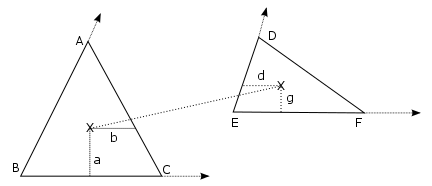
\includegraphics[width=0.6\textwidth]{sketches/c.png}
  \end{center}
  \caption{
    Example of minimum distance and the corresponding barycentric points (parameters of objective function) on a pair of triangles in 3D. Triangle X:T1 has points A, B, C where barymetric parameters a,b correspond to point $x$ on the triangle. Triangle Y:T2 has points D,E,F where barymetric parameters g,d correspond to a point $x$. The two defined barymetric points define the minimum distance between the two triangles in 3D.
  }
  \label{figure:barycentric_contact}
\end{figure}

To enforce the constraints the problem is transformed into a series of unconstrained problems with the augmentation of the objective function $f$ using the penalty-based method. The penalty function penalizes the iteration so that the boundaries of the feasible region are valid. Although there are factors that determine the number of iterations required the tuned-to-the-problem parameters yield a good number of Newton iterations that cannot be reduced to less than two; (initial guess to penalized boundary step, correction step).

\begin{figure}[htb]
  \begin{center}
    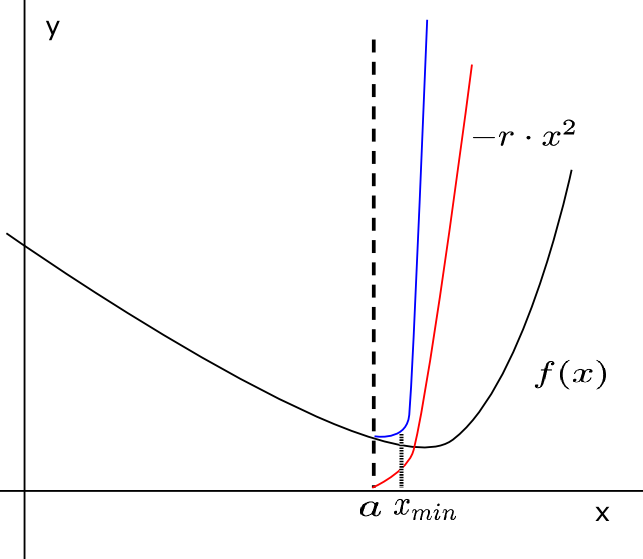
\includegraphics[width=0.5\textwidth]{sketches/penalty.png}
  \end{center}
  \caption{
Illustration of a 2D problem showing the penalty function (red line) penalizing the objective function (black line) f(x) under a constraint $a$ (dash line) to create the feasible region (blue line).
  }
  \label{figure:penaltyfunction}
\end{figure}

This approach adds a penalty term to the objective function to penalize the solution when outside of the feasible region: 
\begin{equation}\label{eq:penalty}
P(x)=f(x)+r\sum_{i=1...6}max(0,c(x_{i}))^{2}
\end{equation}
Where r is the penalty parameter (Figure \ref{}). Newton iterations always converge to a solution slightly on the outside of the feasible region. Convergence can be controlled by the r parameter that controls the sharpness of the curve for the constraints. One aspect that requires care however is the invertibility of the Hessian $\nabla\nabla P$. 

Furthermore the problem is ill conditioned and a Quasi-Newton method is used. The Hessian matrix is not invertible so it is not possible to solve the direction of the search by computing the Hessian and gradient. This illustrates the fact that $f$ has multiple minima and $\nabla\nabla f$ is singular. Consequently, $\nabla\nabla P$ is also singular inside of the feasible region. The ill conditioning is caused by the problem definition itself, where there is a state where there are multiple solutions to the problem based on the orientation of the two triangles. This is also revealed by the two zero eigenvalues of the Hessian. Because of the ill-conditioning, we use a quasi-Newton approach, where the Hessian is approximated by a perturbed operator $\nabla\nabla P + \epsilon I$. $I$ is an identity matrix and $\epsilon$ is suitably small.

\begin{algorithm}
	\protect\caption{\label{alg4}Penalty Solver.}
	\begin{algorithmic}[1]
	
	\Function{Penalty}{A, B, C, D, E, F, rho, tol}

		\State $BA~=~B-A;~CA~=~C-A;~ED~=~E-D;~FD~=~F-D;$

		\State $hf~=~{[}2{*}BA{*}BA',~2{*}CA{*}BA',-2{*}ED{*}BA',-2{*}FD{*}BA';$

		\State $2{*}BA{*}CA',~2{*}CA{*}CA',-2{*}ED{*}CA',-2{*}FD{*}CA';$

		\State $2{*}BA{*}ED',-2{*}CA{*}ED',~2{*}ED{*}ED',~2{*}FD{*}ED';$

		\State $2{*}BA{*}FD',-2{*}CA{*}FD',~2{*}ED{*}FD',~2{*}FD{*}FD'{]};$

		\State $x~=~{[}0.33;~0.33;~0.33;~0.33{]};$

		\For{i=1:99}

			\State $X~=~A+BA{*}x(1)~+~CA{*}x(2);$

			\State $Y~=~D+ED{*}x(3)~+~FD{*}x(4);$

			\State $gf~=~{[}2{*}(X-Y){*}BA';~2{*}(X-Y){*}CA';~-2{*}(X-Y){*}ED';~-2{*}(X-Y){*}FD'{]};$

			\State $h~=~{[}-x(1);~-x(2);~x(1)+x(2)-1;~-x(3);~-x(4);~x(3)+x(4)-1{]};$

			\State $dh~=~{[}-1,~0,~1,~0,~0,~0;~0,~-1,~1,~0,~0,~0;$

			\State $0,~0,~0,~-1,~0,~1;~0,~0,~0,~0,~-1,~1{]};$

			\State $mask~=~h'~$>$=~0;$

			\State $dmax~=~dh.{*}~{[}mask;~mask;~mask;~mask{]};$

			\State $gra~=~gf~+~rho~{*}~dmax~{*}~max(0,h(:));$

			\State $hes~=~hf~+~rho{*}dmax{*}dmax'~+~eye(4,4)/rho^2;$

			\State $dx~=~hes\textbackslash{}gra;$

			\State $DX~=~BA{*}dx(1)~+~CA{*}dx(2);$

			\State $DY~=~ED{*}dx(3)~+~FD{*}dx(4);$

			\State $error~=~sqrt(DX{*}DX'+DY{*}DY');$

			\If{error~$<$~tol}
				\State $BREAK;$
			\EndIf

			\State $x~=~x~-~dx;$

		\EndFor

	\EndFunction
	\end{algorithmic}

\end{algorithm}


The penalty algorithm as shown in Algorithm \ref{} accepts A, B, C, D, E, F vector coordinates for triangle T1(A, B, C), T2(D, E, F) as well as the required parameters for the algorithm to be solved. Rho is the penalty parameter that controls the steepness of the P(x) function (equation \ref{eq:penalty}) , eps is the perturbation parameter for the hessian matrix of the problem along its diagonal to make the matrix solvable. Tol is the tolerance for convergence (Floating point accuracy). In line 23 of Algorithm \ref{} an initial guess is chosen to be the center of the two triangles, then the for loop initiates the Newton iterations to find the points on the X, Y triangle planes under the constraints c. For each of the six constraints (line 12) the max function of the penalty is determined so that every possible active constraint is detected. In line 17 and line 18 the gradient and Hessian of P Penalty function is evaluated to be provided to the Gaussian elimination direct solver so that a Newton direction DX is solved. If the Newton step is large enough over the specified tolerance then the iteration is converged else the direction is used and the loop is executed once more recursively.

The penalty method is well-suited for SIMD optimisation because we can concurrently determine the distance between multiple triangle pairs as long as we use the same number of Newton steps: Up to four or eight
triangle pair distances can be determined at the same time; depending on the vector width. Such a speed-up statement however has to be read carefully. While the concurrency is high, it is not clear a priori how many Newton steps are required. A high number of Newton steps can render the penalty method slower than the brute force approach.
\subsection{Hybrid approach}
To create a hybrid solver we first assume that on average there are for each triangle pair distance computation only a few iterations that are required to arrive to a solution \ref{}. Based on empirical studies and tuning of the penalty parameter and the regularization variable, the majority of triangle pairs are solved within four iterations as shown in Figure {}. Secondly we set a user defined tolerance of error to the method to act as the switching point for the falling-back to brute force solver. If the number of fall backs does not overtake the number of penalty-based solutions then the method is a compromise between brute force and penalty both in terms of performance but also in terms of error of solution. 

\begin{figure}[htb]
  \begin{center}
    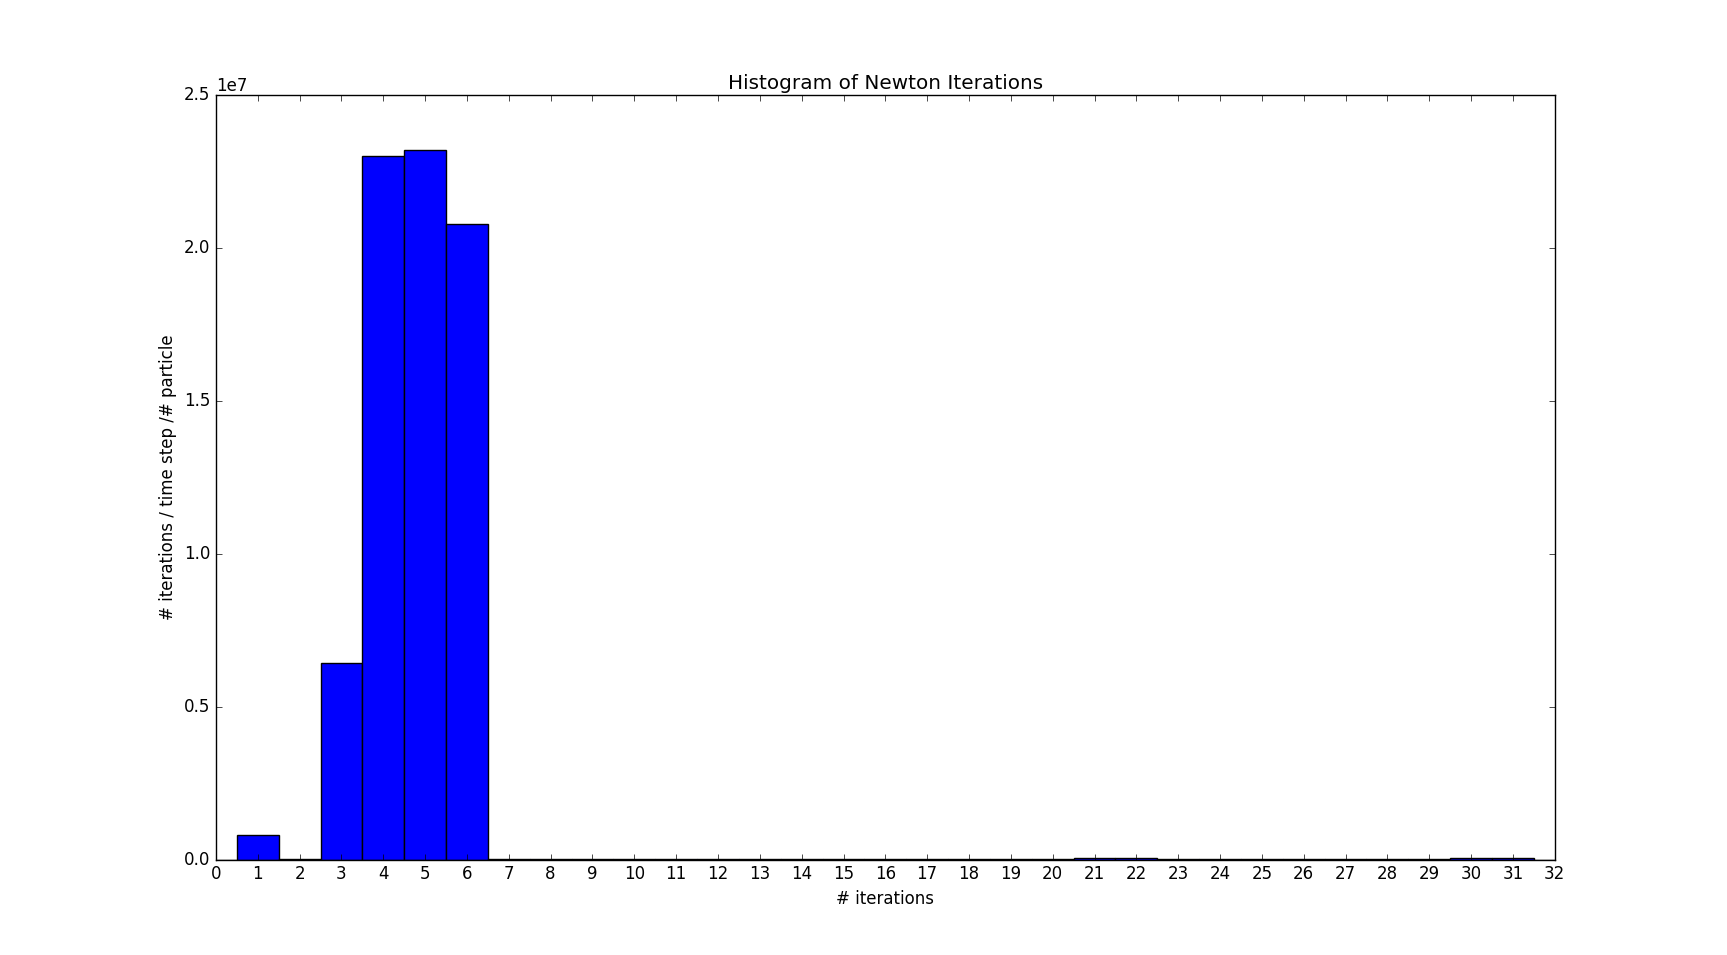
\includegraphics[width=1\textwidth]{experiments/random/penalty-stats/bar.png}
  \end{center}
  \caption{Histogram of number of iterations required by Newton Method for convergence on a sample of twenty four million triangle pair configurations.}
  \label{figure:newton_hist}
\end{figure}

There are two variants of hybrid method; the first is the hybrid-on-triangle-pairs and the second one is hybrid-on-triangle-batches. Both variants are developed to exploit the robustness of brute force while keeping the arithmetic intensity of the penalty method. The implementation of both methods takes into account the potential for shared memory scaling as well as data access continuity. In addition SIMD vectorised performance of the underlying methods and memory alignment are critical for the execution of both methods.

The first variant is hybrid-on-triangle-pairs where it divides the computational workload to be per each triangle pair. The hybrid-on-triangle-pairs method runs first the penalty solver on one triangle pair, if the solution is not within the user specified tolerance, we fall back to brute force to solve the problem naively. 

\begin{algorithm}
 \caption{Hybrid On Triangle Pairs} \label{algorithm:hybridTriangle}
 \begin{algorithmic}[1]

	\Function {hybridOnTrianglePairs(particleA, particleB, tolerance)}	
	
		\For {i = 0 to n particleA.triangles}
	
			\For {j = 0 to n particleB.triangles}
			
				\State {triangleError = penalty(particleA[i], particleB[j])}

				\If {triangleError > tolerance}

					\State {bruteForce(particleA[i], particleB[j])}
	
				\EndIf
	
			\EndFor
			
		\EndFor
		
		\Return {P, Q points on two triangles}
	
	\EndFunction
	
 \end{algorithmic}
\end{algorithm} 

The other variant is the hybrid-on-batches where it is hybrid per triangle batches. This method is checking the error less frequently than the previous variant and uses an error for the whole batch. As in the hybrid-on-triangle-pairs variant; we run then penalty method on one batch of triangles and then fall back to brute on the whole batch if the error tolerance is not satisfied. The batch size can be set by the user to be of any arbitrary size. For our application we set it to be the number of triangles of our non-spherical particles (tessellation size of 60~ triangles).    

\begin{algorithm}
 \caption{Hybrid On Triangle Batches} \label{algorithm:hybridBatches}
 \begin{algorithmic}[1]
	
	\Function {hybridOnTrianglePairs(particleA, particleB, tolerance)}	
	
		\For {i = 0 to n particleA.triangles}
	
			\For {j = 0 to n particleB.triangles (batchSize)}
					
				\State {batchError = penalty(particleA[i], particleB[j])}

			\EndFor
			
			\If {batchError > tolerance}
				
				\For {j = 0 to n particleB.triangles}
	
					\State {bruteForce(particleA[i], particleB[j])}

				\EndFor
	
			\EndIf
	
		\EndFor
	
		\Return {P, Q points on two triangles}	
	
	\EndFunction
	
 \end{algorithmic}
\end{algorithm} 

Both hybrid methods suffer by their nature by the granularity of the grain size whether that is singular size (triangle pair) or greater (batches of pairs).
The memory distribution of pairs of triangles that do not converge within the mean number of Newton iterations are not known a priori because the solution depends on the underlying geometry. Triangle pairs or triangle batches that do not converge within the set tolerance skew the overall error distribution margin, potentially creating the worse case scenario where the method becomes a worse than brute force solver with both penalty and brute force being executed in sequence. It is not possible to predict the sparsity/distribution of non-convergent triangle pairs/batches during run-time so the tolerance value, penalty, regularization parameters are vital. In our experiments those parameters are set based on empirical tuning and trial and error.



\section{Shared memory parallelisation}
\label{section:shared-memory}

We introduce three levels of shared memory parallelisation. On the highest level, we exploit the cell level decomposition and assign work within each cell to cores. Within the cell we assign work per particle pair  to an inner fork-level of threads. Lastly within each particle pair the innermost level of parallelisation is utilised to exploit tessellation level parallelisation by the contact solver.

Three levels of multicore parallelisation:

a) on the cell level
b) within one 'cell' do all the particles in parallel
c) within one particle-particle sweep, do all the triangles in parallel

%describe the setup
For the multi-core scaling experiments we setup runs that use the hybrid solver and the brute force solver. We base performance experiments on three main runtime setups. We use meshed non-spherical particles of approximately 60 triangles each based on the Delauny triangulation (see appendix) derived from a 50 sphere shaped point cloud. We scale the contact problem in two aspects; by number of non-spherical particles and by irregularity of particle radius size. We use regular grid, adaptive and reluctant grids for grid-based adaptivity. Lastly, the particles mass is homogeneous to the particles and the initial velocities are random for every particle. To enhance the time to solution we use spheres as a last stage boundary box to minimize the number of mesh to mesh contact solving per timestep per cell per vertex.

\clearpage

In the innermost level of parallesation we are experimenting with several solver methods to resolve contact points. At this level computation is parallelised based upon triangle pairs and triangle batches and assigned to threads statically. 
From the performance measurements in Figure \ref{figure:triangle_omp} it is observed that Hybrid-on-triangle-pairs scales but it is slowest method to solution per timestep. 

\begin{figure}[htb]
  \begin{center}
    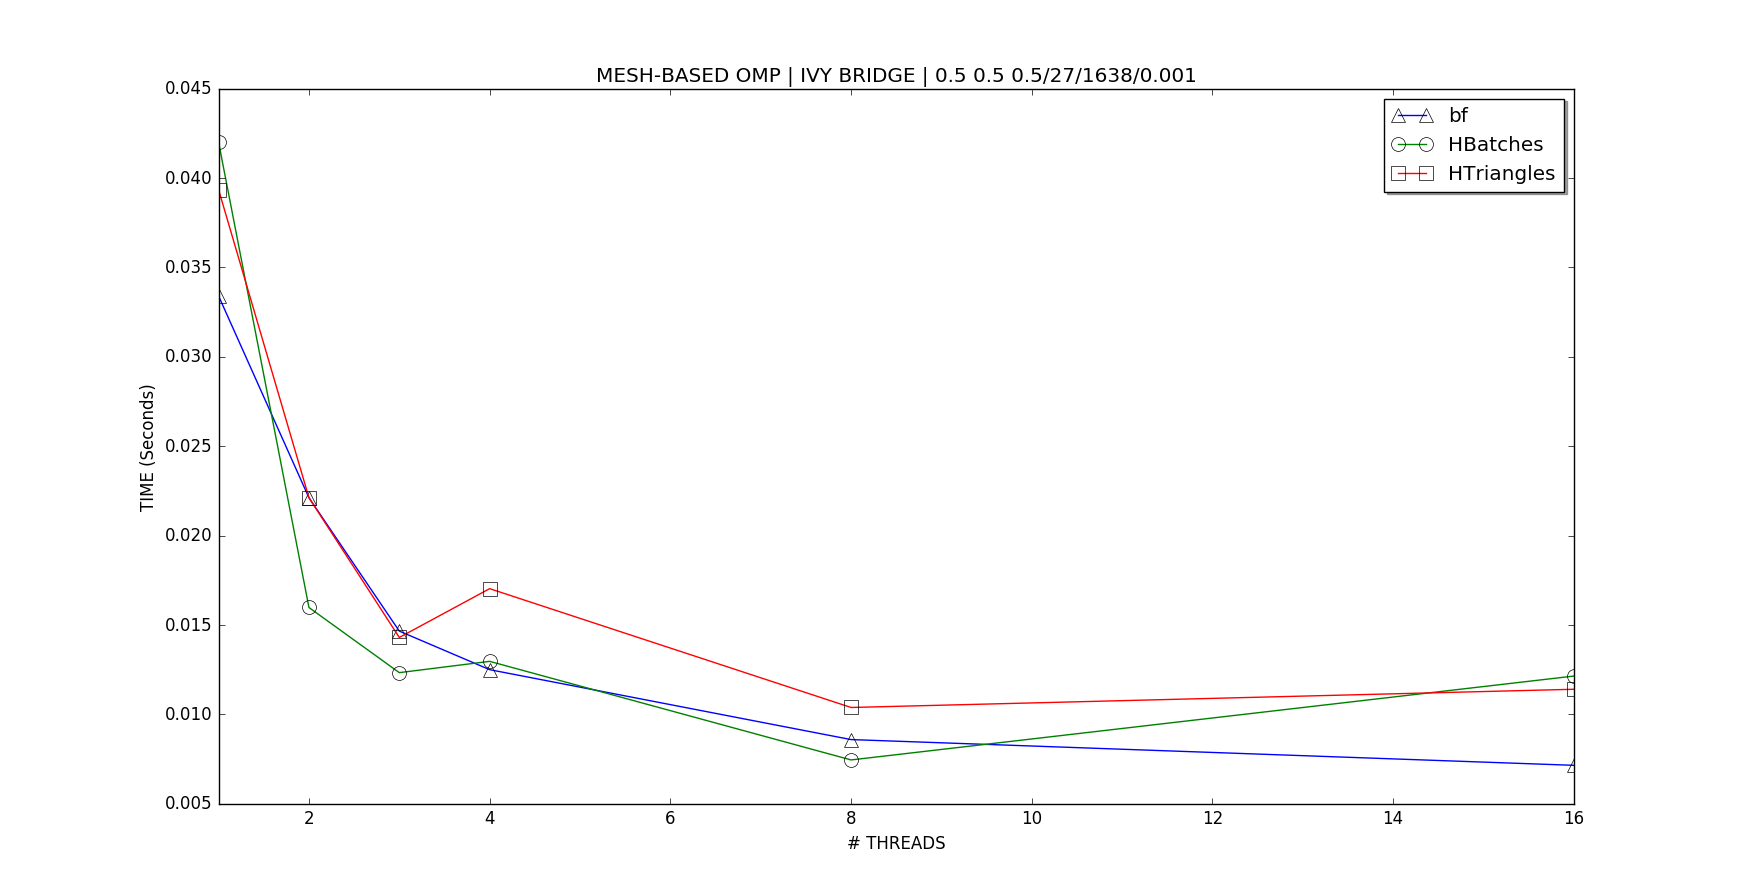
\includegraphics[width=0.8\textwidth]{experiments/random/omp/triangle_based_x0.png}
  \end{center}
  \caption{Triangle based shared memory parallelism using openMP running brute force (bf), hybrid-on-batches (HBatches) and hybrid-on-triangle-pairs (HTriangles) methods.}
  \label{figure:triangle_omp}
\end{figure}

\begin{figure}[htb]
  \begin{center}
    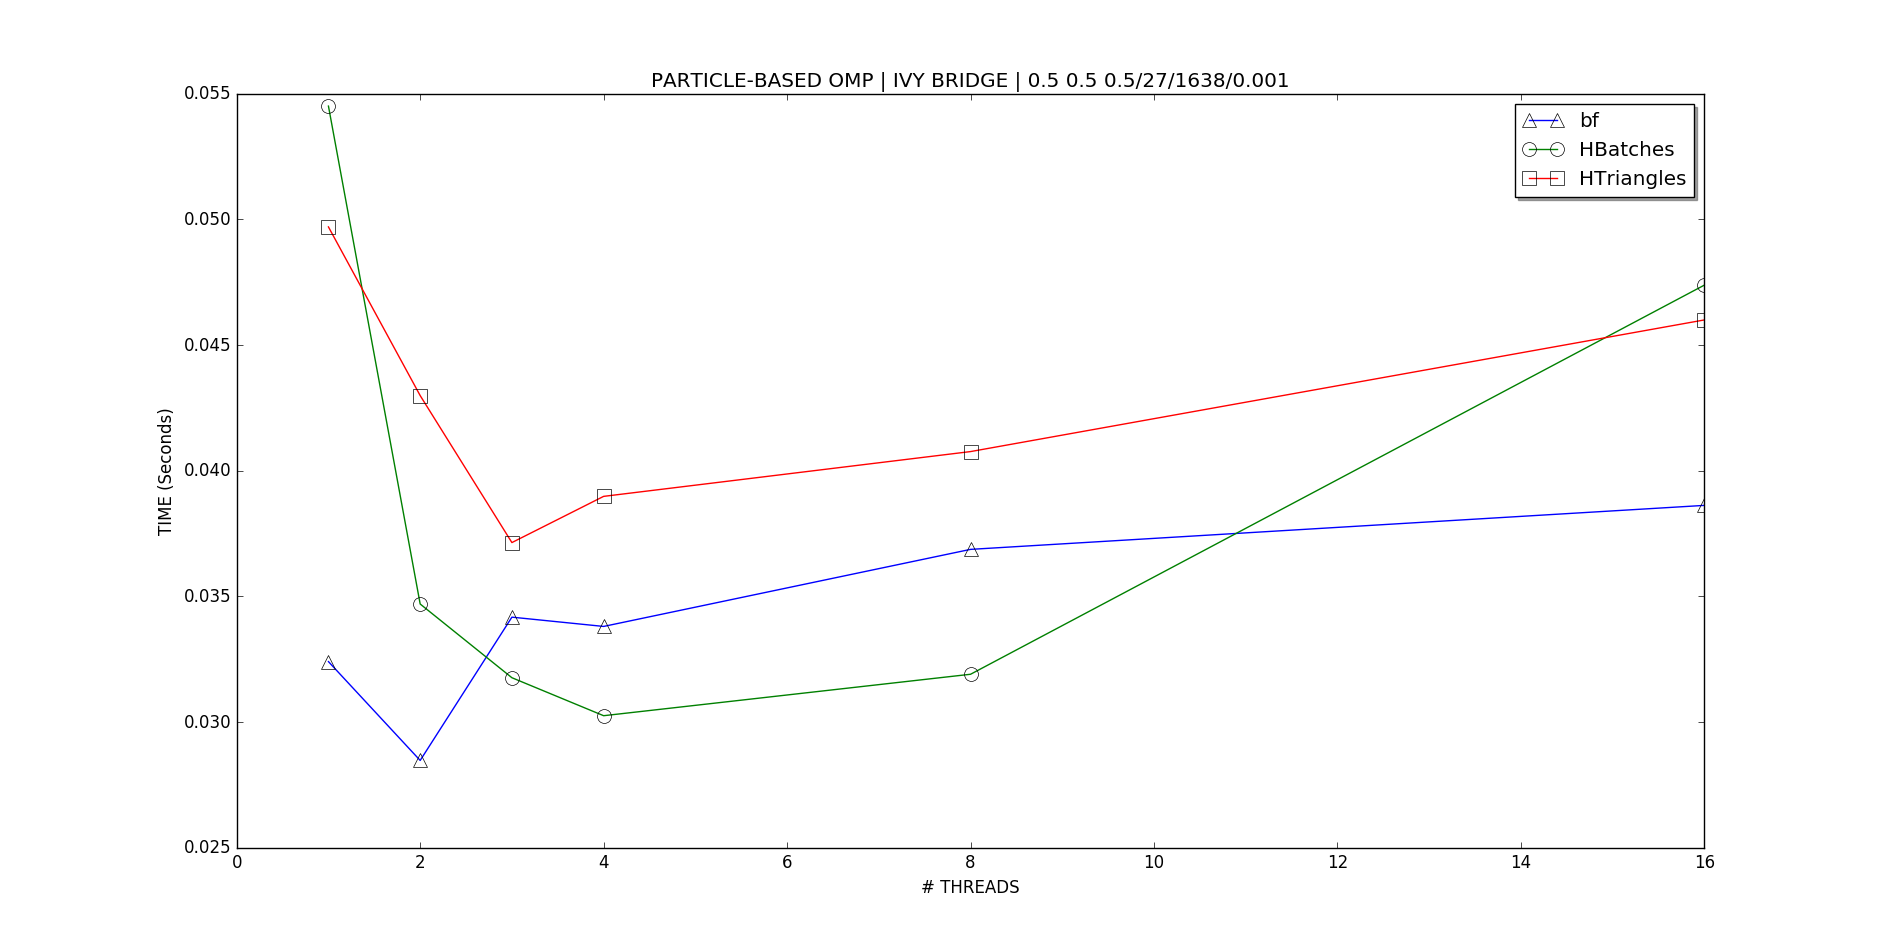
\includegraphics[width=0.8\textwidth]{experiments/random/omp/particle_based_x0.png}
  \end{center}
  \caption{Particle based shared memory parallelism using openMP running brute force (bf), hybrid-on-batches (HBatches) and hybrid-on-triangle-pairs (HTriangles) methods.}
  \label{figure:particle_omp}
\end{figure}

The alternative method of parallelisation is based on whole particle pairs. Thread subscription is performed during the outer sweeping of particles where pairs-of-particles per grid-vertex are computed in parallel on each vertex visit. In Figure \ref{figure:particle_omp} we see that again hybrid-on-triangle-pairs is performing worst and hybrid-on-batches to scale better. Brute force does not scale as well as hybrid-on-batches but has faster time to solution on low number of threads.

\begin{figure}[htb]
  \begin{center}
    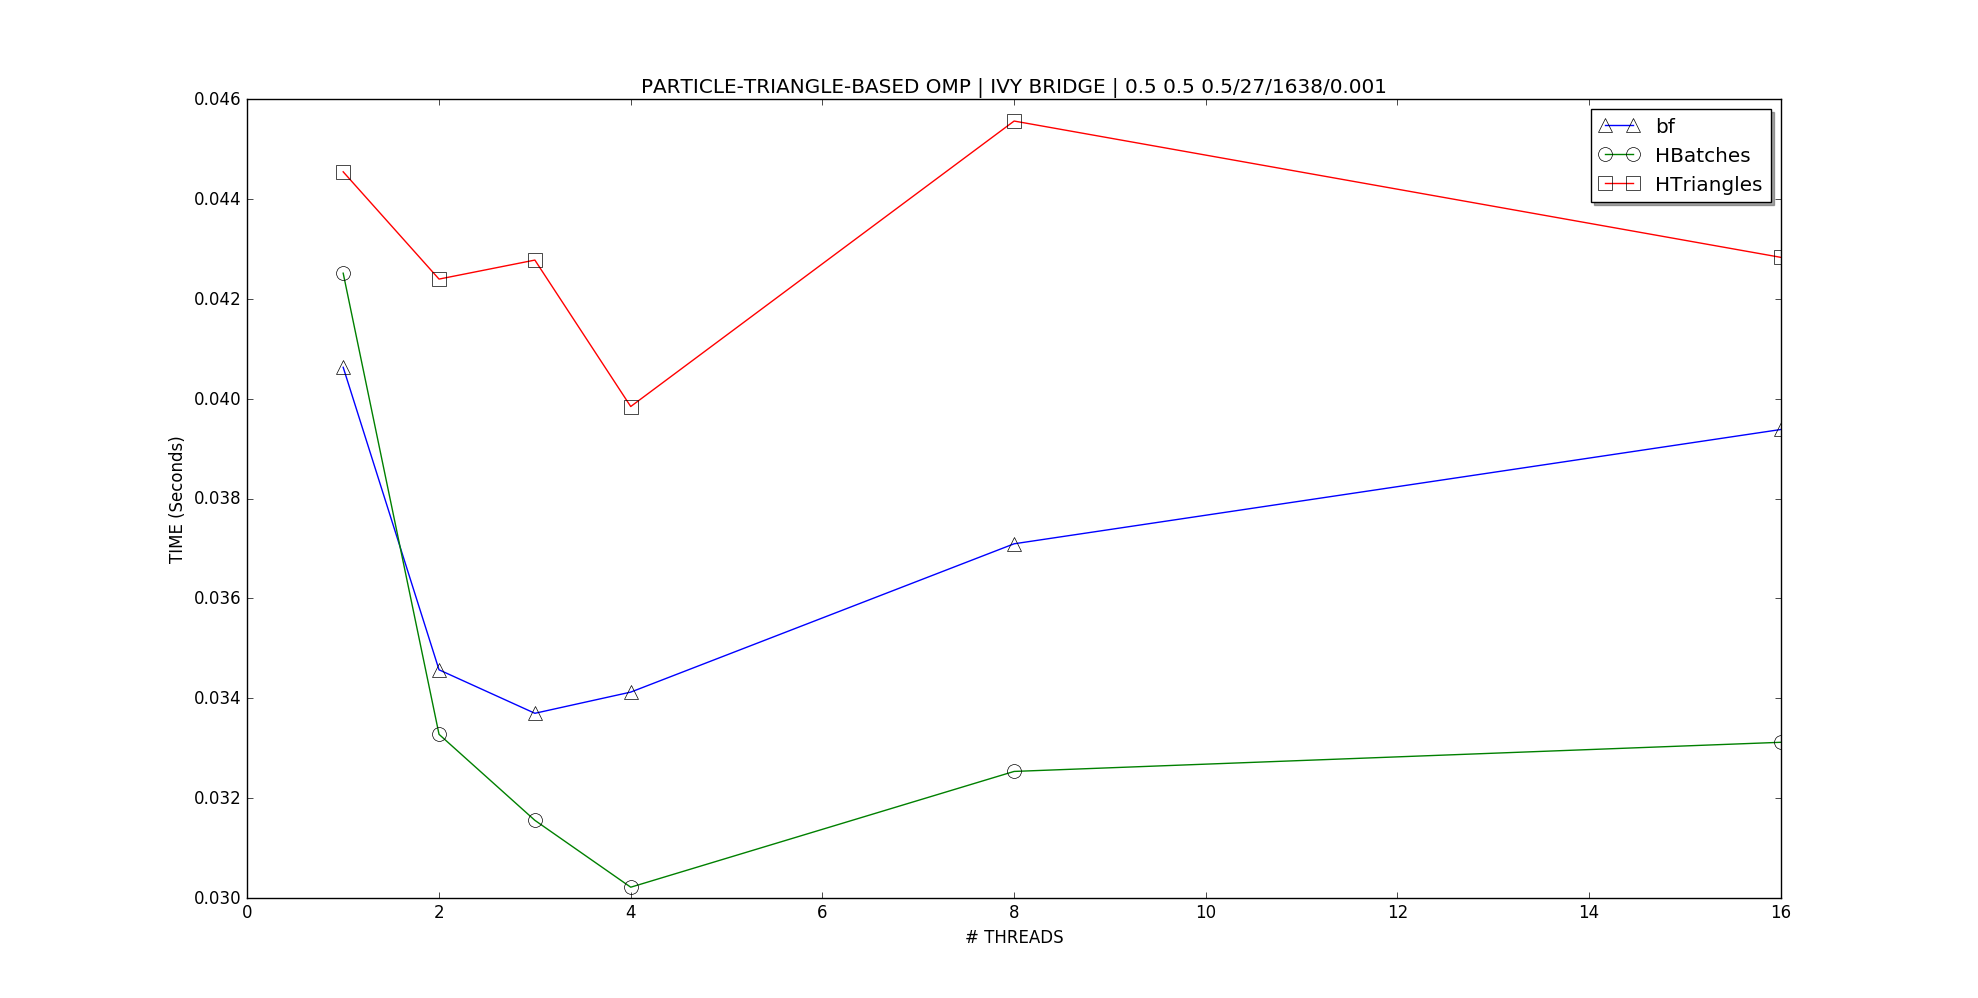
\includegraphics[width=1\textwidth]{experiments/random/omp/particle_triangle_based_x0.png}
  \end{center}
  \caption{Particle and Triangle based nested shared memory parallelism using openMP running brute force (bf), hybrid-on-batches (HBatches) and hybrid-on-triangle-pairs (HTriangles) methods.}
  \label{figure:particletriangle_omp}
\end{figure}

Particle and Triangle parallelism nests both particle and triangle shared memory threads. The runtime to solution is slightly slower than particle-based parallelism due to the thread/openMP overhead. Nevertheless it has an impact on brute-force method as it scales smoother than particle-based only parallelism due to overhead. In this case hybrid-on-batches is also the fastest while the hybrid-on-triangle-pairs the slowest. 

\clearpage

\begin{figure}[htb]
  \begin{center}
    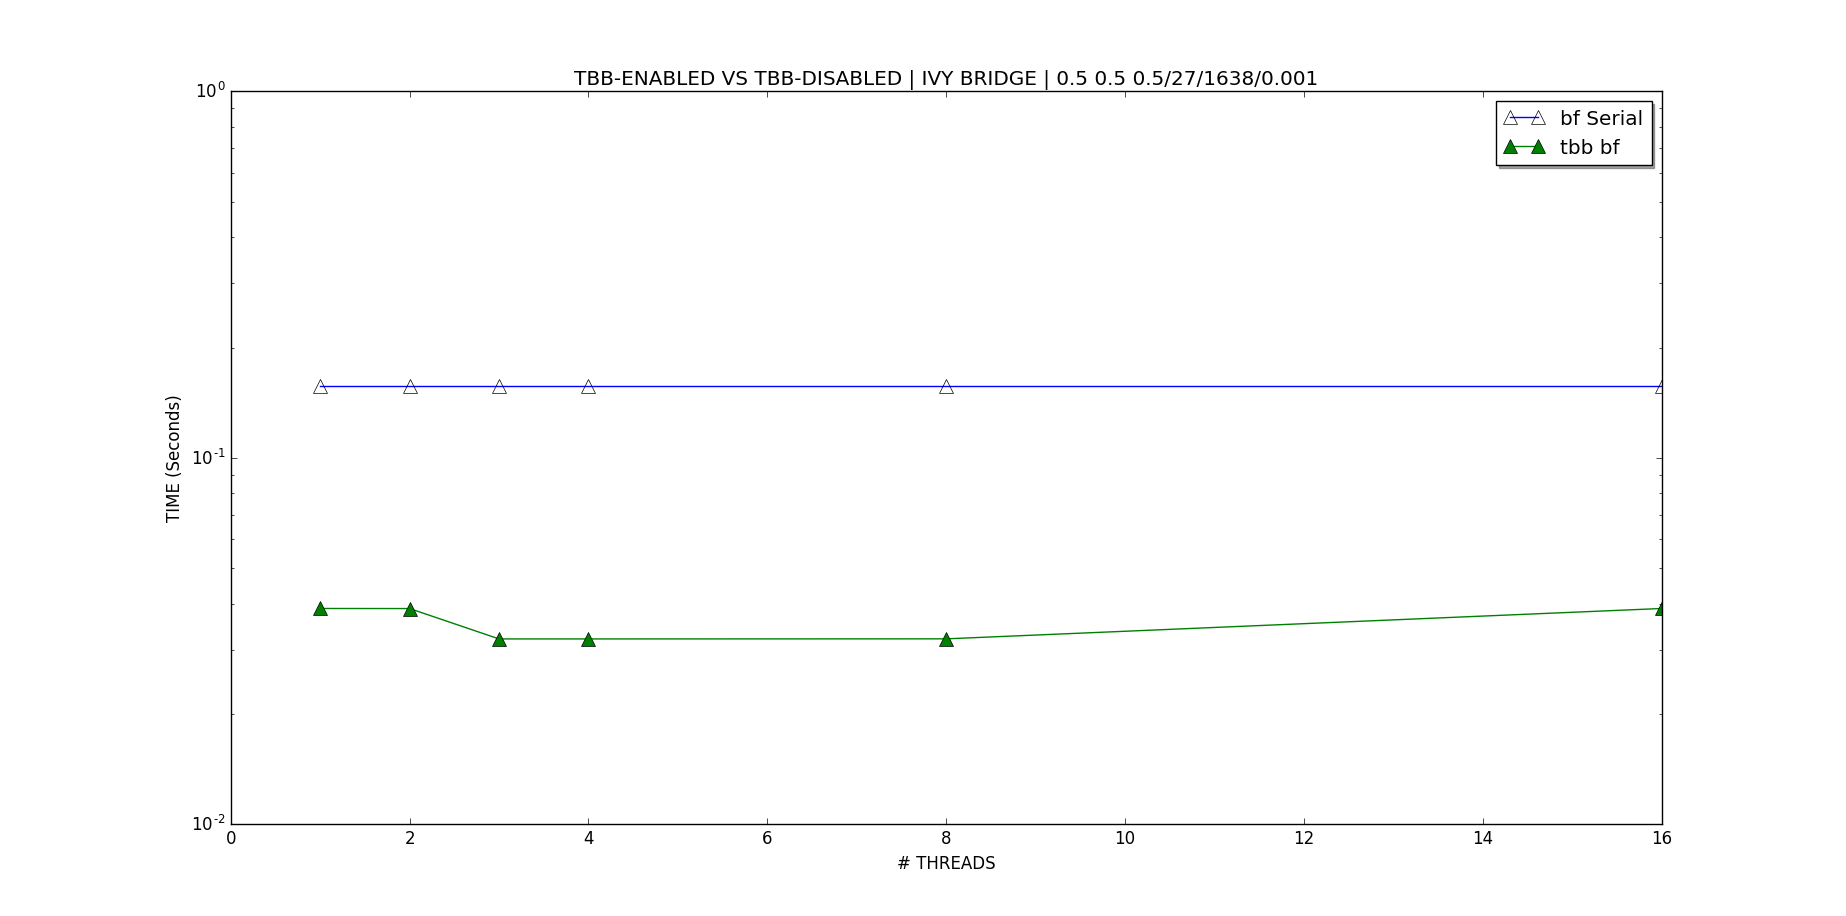
\includegraphics[width=1\textwidth]{experiments/random/omp/tbb_vs_serial.png}
  \end{center}
  \caption{Cell based parallelism on Peano compared to serial runs using Intel TBB}
  \label{figure:tbb_vs_serial}
\end{figure}

Another aspect of shared memory performance is thread scheduling and balancing implications.
The non-deterministic nature and error-prone distribution of triangles of the hybrid algorithm as discussed in Chapter {-hybrid chapter-} would suggest that alternative scheduling would pay off. But for our experiments dynamic and guided thread scheduling didn't not have a performance improvement on our tests but they rather create an scheduling overhead instead. That is partly due to the distribution of error in the triangle pairs and due to the granularity of our batches. Insignificant improvements were shown to our worst hybrid-on-triangle-pair method when using dynamic scheduling with OpenMP on the ivy bridge machine.    

At the highest level of shared memory parallelism is the grid cell-based multicore processing. It is based on the peano-framework that is using Intel TBBs to assign cells on threads. This has significant impact on the overall runtime performance in Figure \ref{figure:tbb_vs_serial} it is compared with plain serial execution. Number of threads on the x axis refer to TBB Cell-based threads, at the contact detection method level the computation is performed without shared memory parallelism but with vectorization enabled. For the specified experiment in Figure {} we observe no cell-based thread scaling but only reduction of time to solution. But when we increase the problem size further (figure \ref{figure:tbb_scaling}) we see that cell-based parallelism scales and it enhances execution time. 

\begin{figure}[htb]
  \begin{center}
    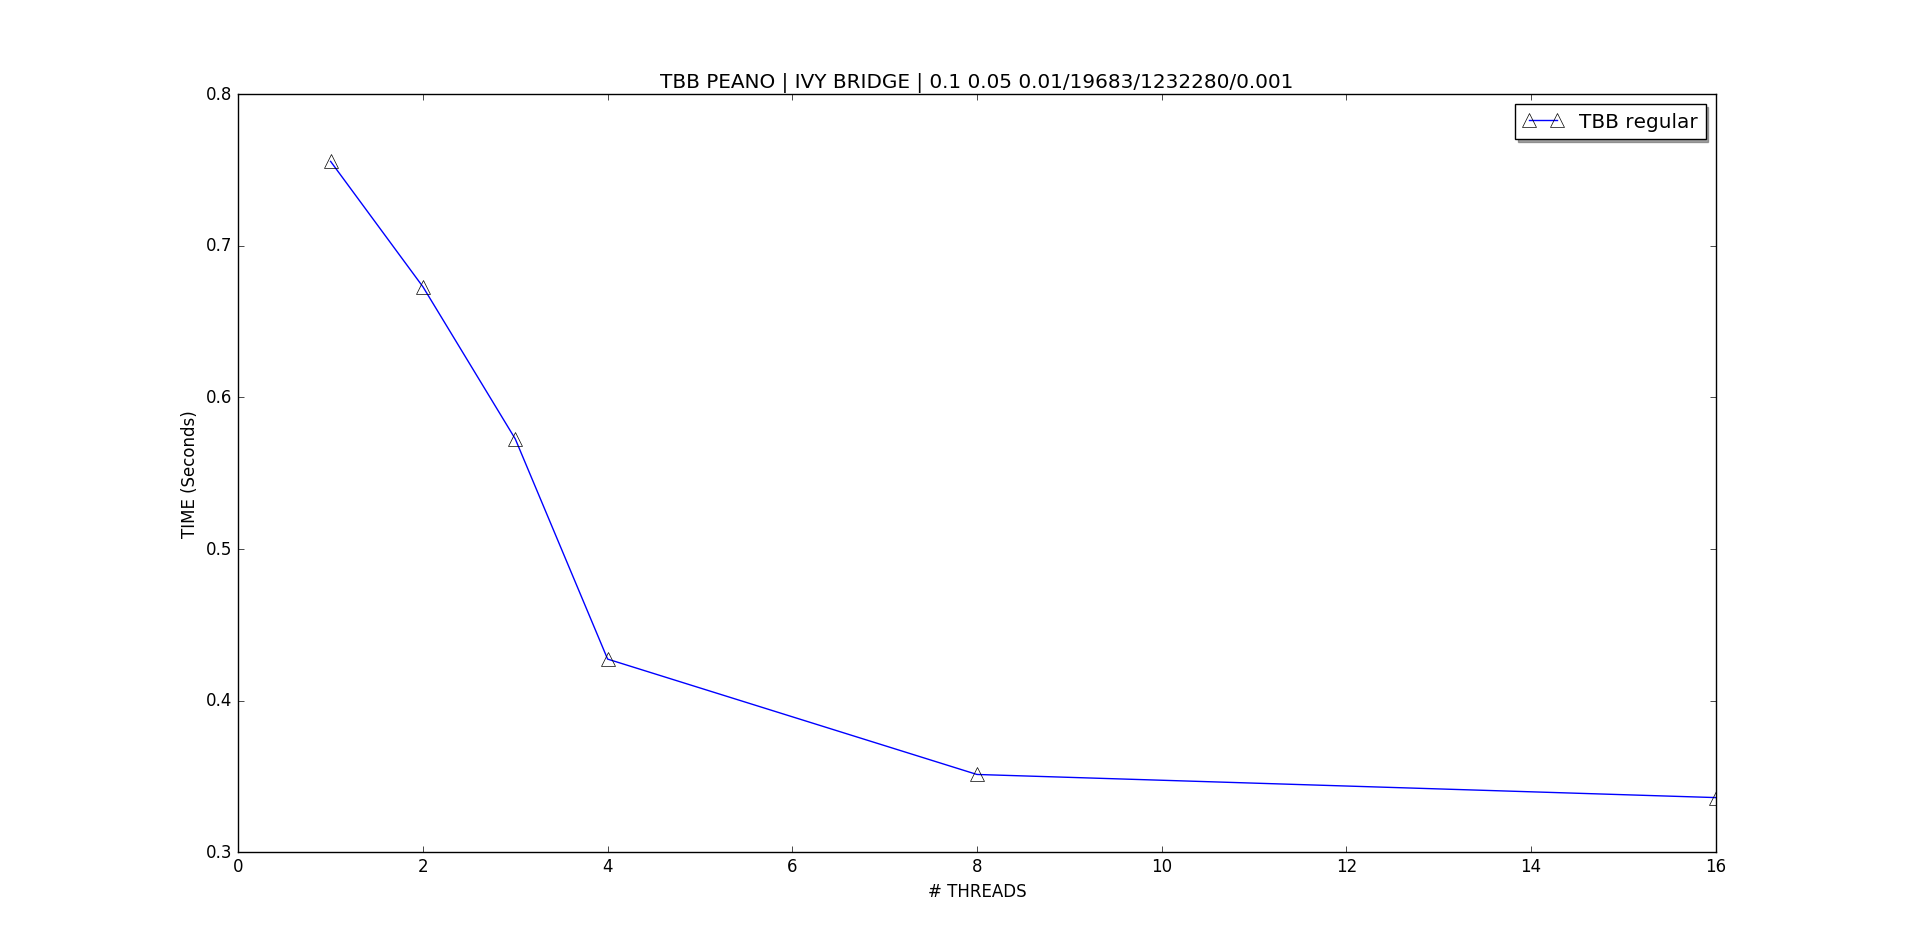
\includegraphics[width=0.8\textwidth]{experiments/random/omp/tbb_regular_x2.png}
  \end{center}
  \caption{Cell based parallelism on Peano compared to serial runs using Intel TBB}
  \label{figure:tbb_scaling}
\end{figure}

Overall shared memory parallelism on these three levels of parallelisation yield performance gain on manycore systems for our hybrid-on-batches method and in some cases brute force. For small problems triangle-based parallelism show good time to solution but for larger (**put plot) problem sizes particle-based parallelism pays off better. The finer/inner the thread forking the less significant scaling it is observed for larger problem sizes. For large problem sizes the combination of cell-based plus particle-based multi-core parallelism using hybrid-on-batches makes sense. Furthermore additional overall speedup can be gained if spheres are used as a filtering bounding box stage to our triangle-to-triangle contact detection.

\clearpage


\section{Performance results}
\label{section:results}

We study the behaviour of our algorithms at hands of an artificial granulate
setup. 
Granulates of various diameters between $diam_{min}$ and $diam_{max}$ are
randomly distributed in a unit cube.
They are assigned random velocity and fixed density. 
If particles bump into the unit cube wall, they are reflected by applying an opposite direction in the velocities. 
We apply a full elastic collision model by allowing virtual penetration using the DEM spring-dashpot penalty force function (\ref{xxx}).
Each particle is created by a randomised algorithm that places a random number
of 50 points within the unit sphere. 
We then use the hull algorithm \cite{xxxx} using a Delaunay triangulation to
create the particle that is finally shrinked to fit into the prescribed
diameter.
On average, we obtain around 60-65 triangles per non-spherical particle.


The underlying spacetree is based upon tree-partitioning as we rely on the AMR
framework Peano \cite{Software:Peano}.
All experiments are realised with double precision. 
We note that the combination of the present work with reduced
floating-point accuracy, notably following
\cite{Weinzierl:15:Compression}, however could be advantageous.
All particle velocities and time step sizes $ \Delta t$ are chosen reasonably
small such that particles do never penetrate or jump over more than one grid cell per time step.
Higher velocities require more sophisticated collision models and a more
sophisticated vertex association as discussed in \cite{Weinzierl:16:PIC}.
Particles are assumed to collide as soon as they get closer than $\epsilon =
10^{-8}$.
\marginpar{\footnotesize TW doublecheck $\epsilon $}
Adaptive or implicit time stepping \cite{xxx} are not subject of study.
\marginpar{\footnotesize TK/KK citations}
Two different setups are realised: In the first experiment, we do not imply any
external force.
The particles fly through the unit cube and collide with each other.
In the second experiment, we apply uniform gravity.
The first setup yields an estimate how our code performs if the particle collission
characteristics on the long term is time are invariant while the particle
distribution is instationary.
The second setup yields an estimate how the code performs if particles cluster
and run into a stationary setup.
Both experiments thus cover one extreme of a geometric challenge.


All single node experiments are ran on an Intel Xeon E5-2650 with two times 8
cores running at 2.0 GHz. 
On this system, we use Likwid \cite{Treibig:10:Likwid} to read performance
counters.
All manycore experiments are done on an Intel Xeon Phi 5110P with 8 GByte of
memory running  at 1053 GHz in native mode.
All parallel node experiments are ran on XXX nodes. Parallel experiments are ran on Durham University Hamilton supercomputer where per node there are 2 x Intel Xeon E5-2650 v2 (Ivy Bridge) 8 cores, 2.6 GHz processors, 64 GB DDR3 memory, 1 x TrueScale 4 x QDR single-port InfiniBand interconnect.
We use Intel(R) MPI Library for Linux* OS, 64-bit applications, Version 5.0 Update 3  Build 20150128. 
For performance statements, we rely on the Intel 16 compiler.


%brute force vectorization

\begin{figure}[htb]
  \begin{center}
    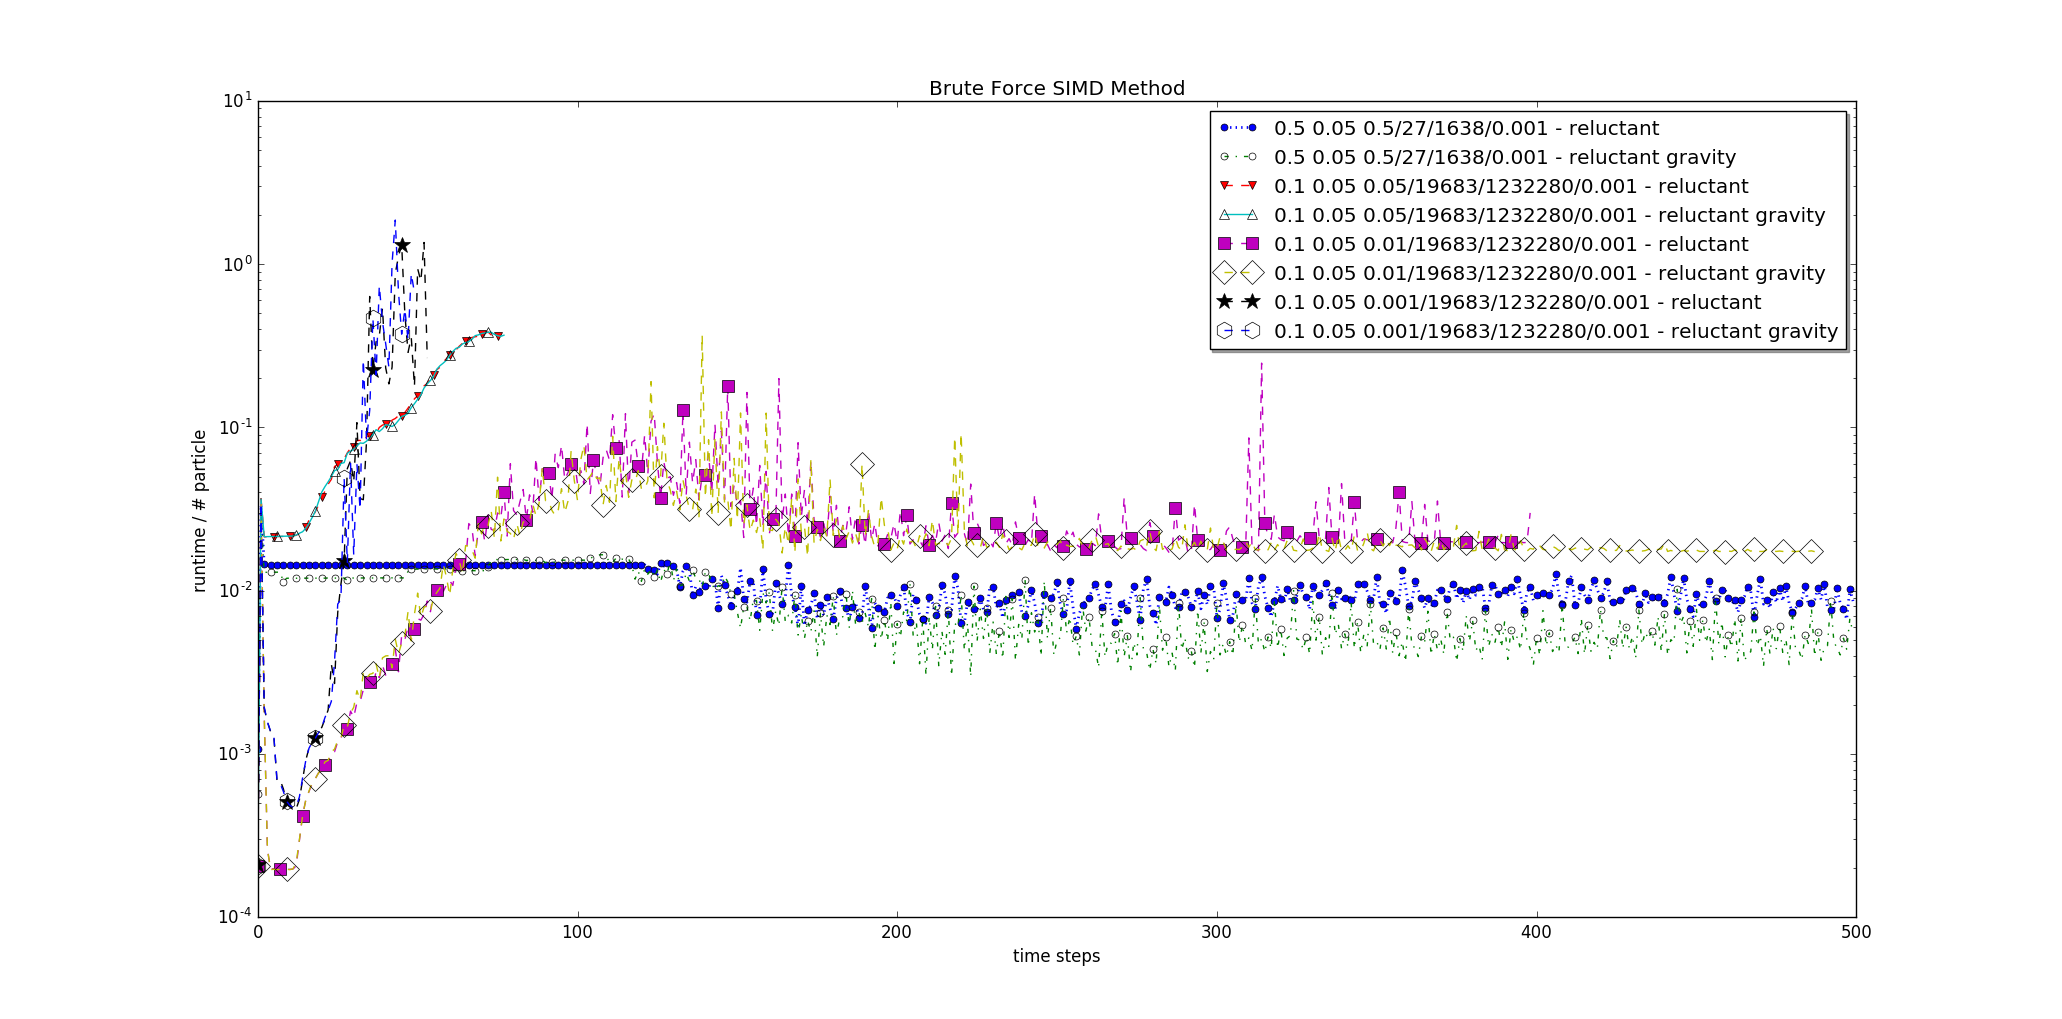
\includegraphics[width=1\textwidth]{experiments/vectorisation/plots/log_bf_simd.png}
  \end{center}
  \caption{Brute Force SIMD runtimes.}
  \label{figure:triangle_omp}
\end{figure}


penalty vectorization

\begin{figure}[htb]
  \begin{center}
    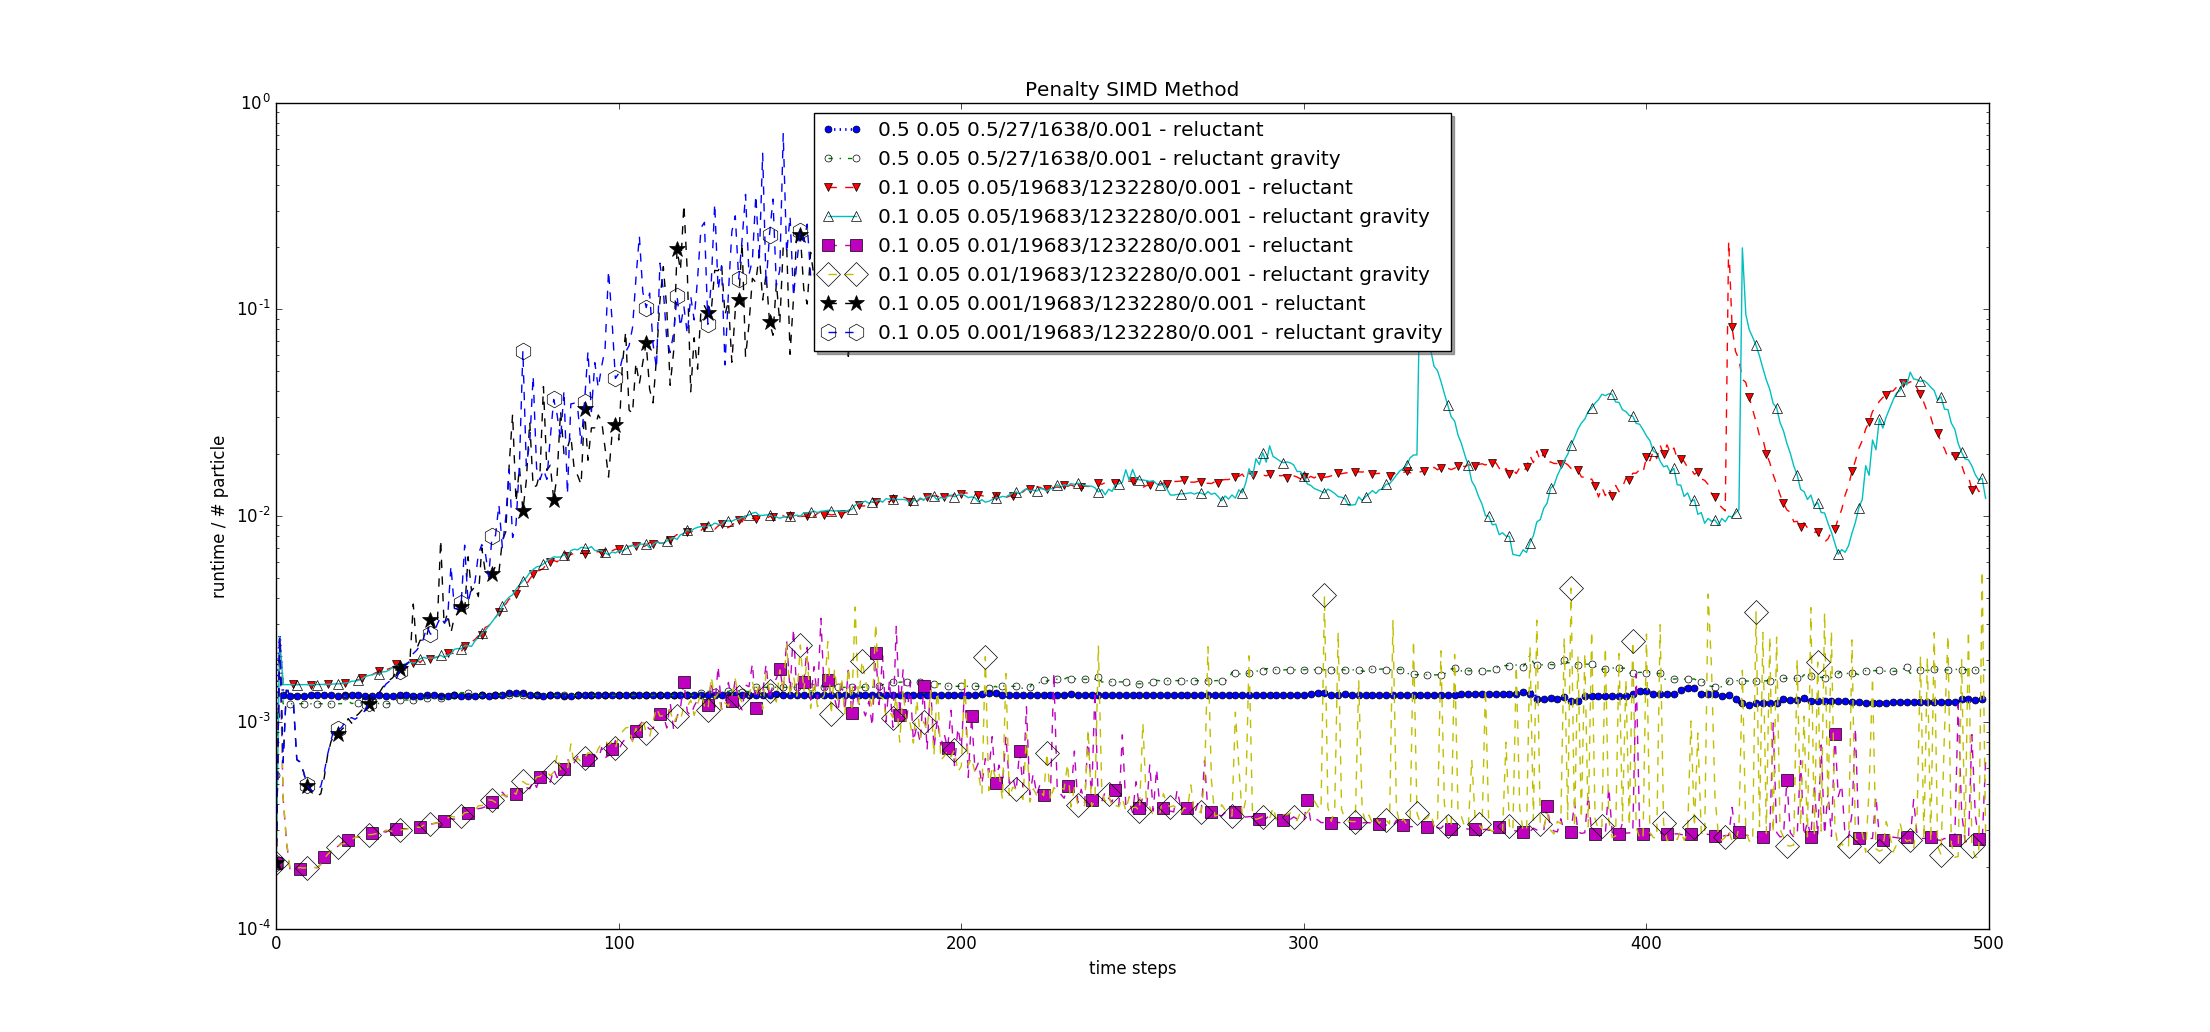
\includegraphics[width=1\textwidth]{experiments/vectorisation/plots/log_penalty_simd.png}
  \end{center}
  \caption{Penalty SIMD runtimes.}
  \label{figure:triangle_omp}
\end{figure}

hybrid vectorization

\begin{figure}[htb]
  \begin{center}
    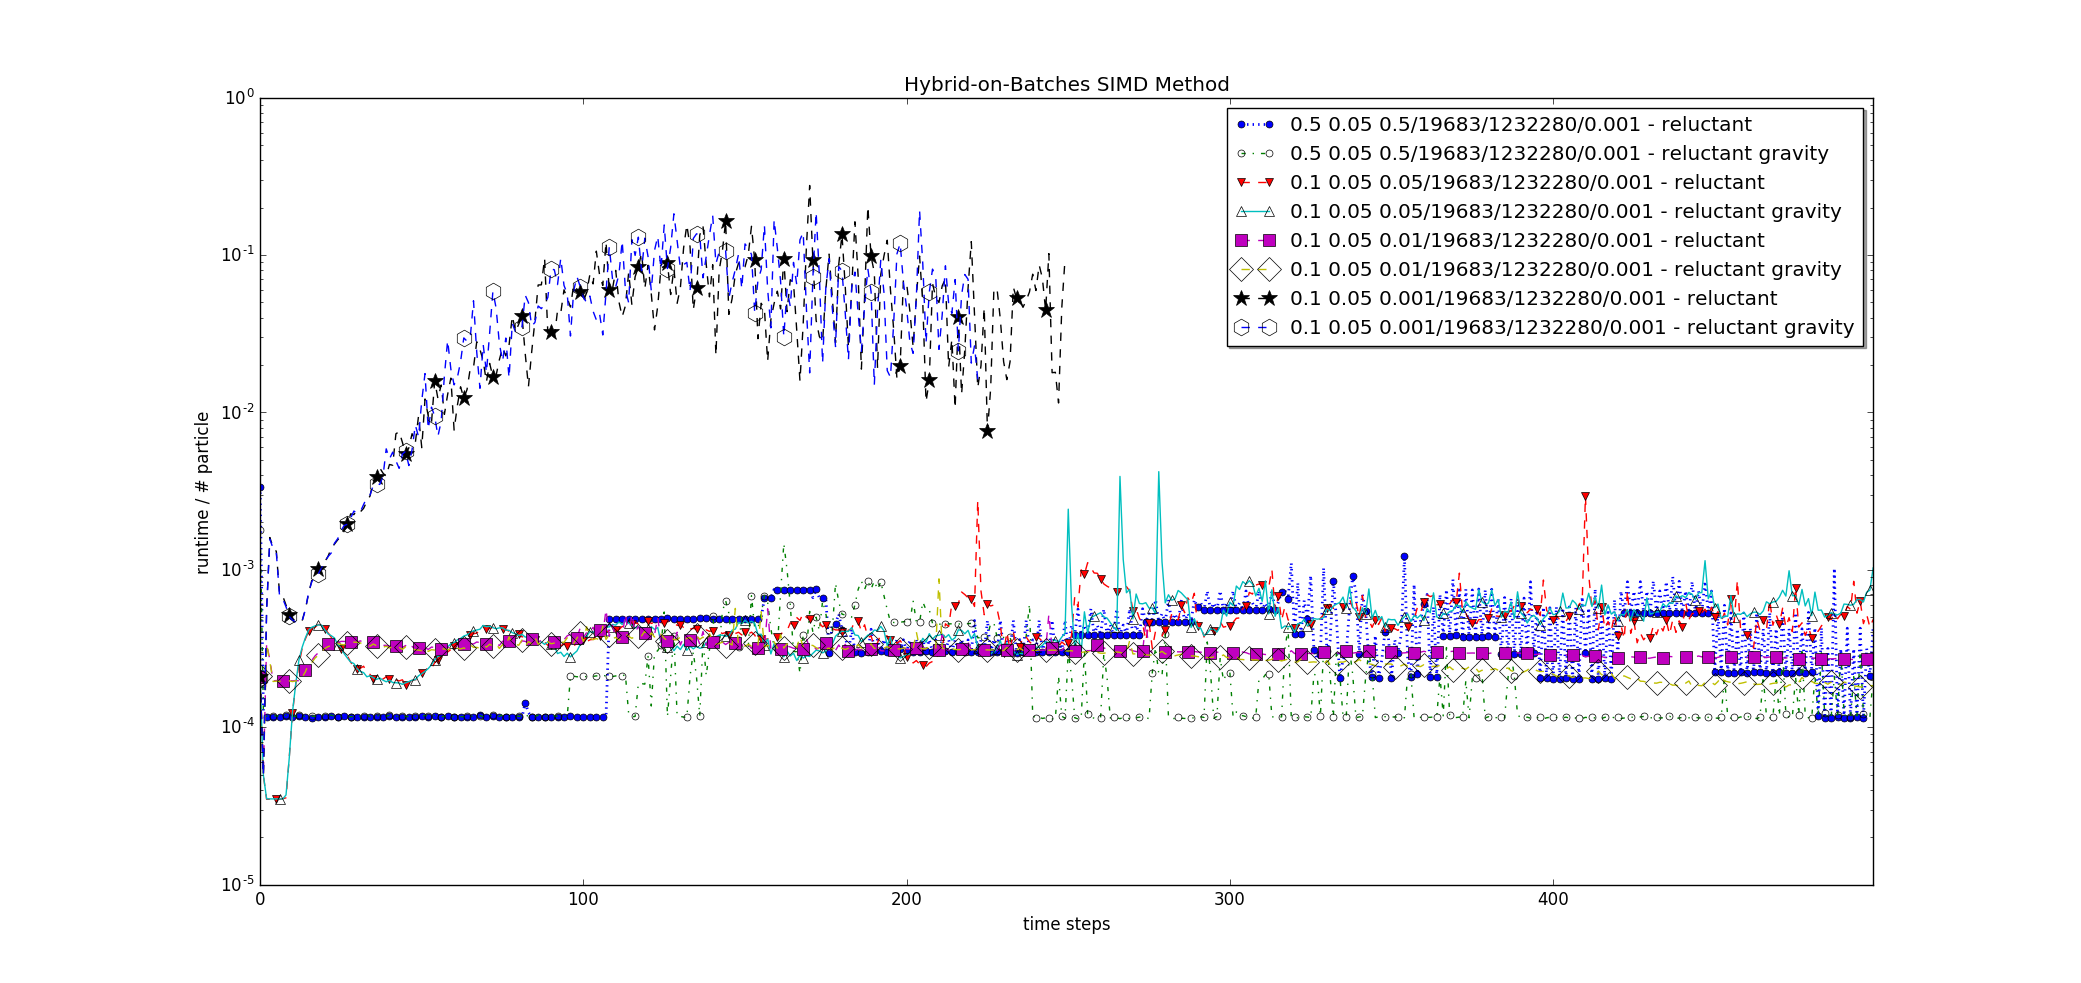
\includegraphics[width=1\textwidth]{experiments/vectorisation/plots/log_sphere-hybrid-on-batchesSIMD.png}
  \end{center}
  \caption{Hybrid-on-batches SIMD runtimes.}
  \label{figure:triangle_omp}
\end{figure}


\begin{figure}[htb]
  \begin{center}
    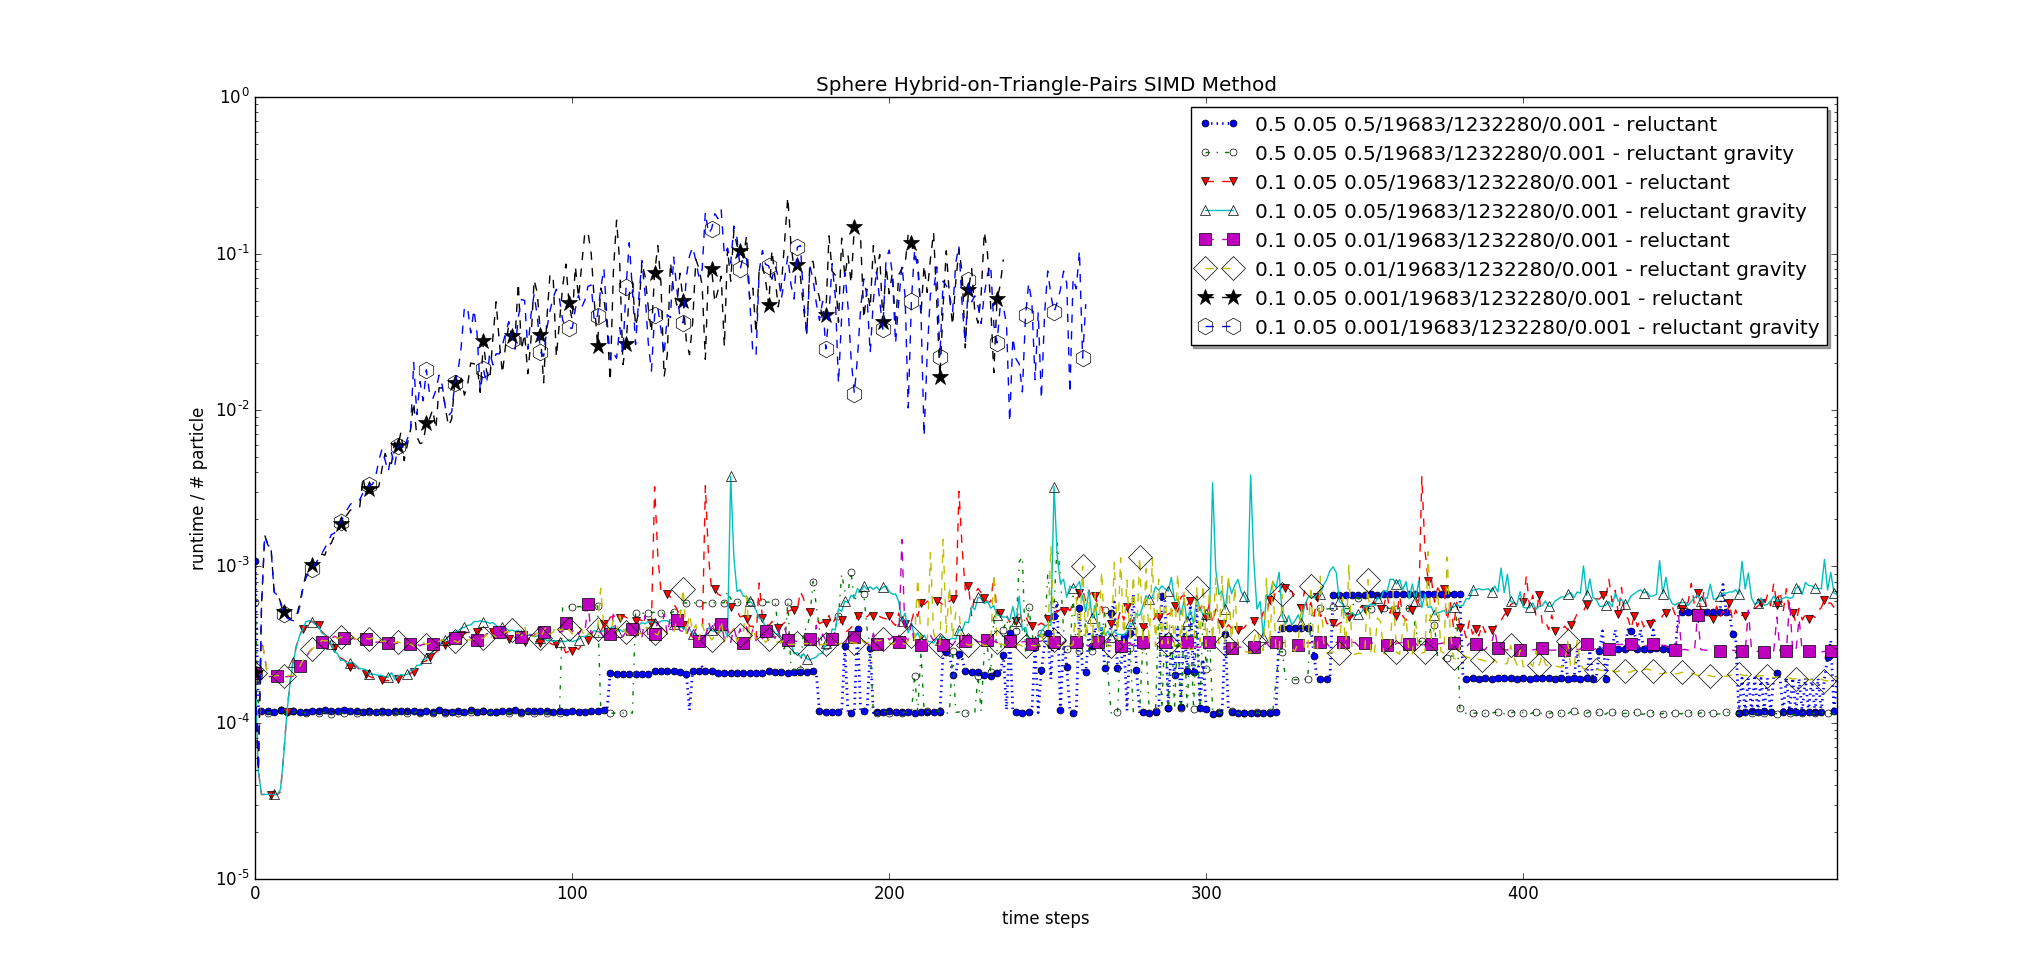
\includegraphics[width=1\textwidth]{experiments/vectorisation/plots/log_sphere-hybrid-triangle-pairs-SIMD.png}
  \end{center}
  \caption{Hybrid-on-triangle-pairs SIMD runtimes.}
  \label{figure:triangle_omp}
\end{figure}

overall vectorization speedup
\begin{figure}[htb]
  \begin{center}
    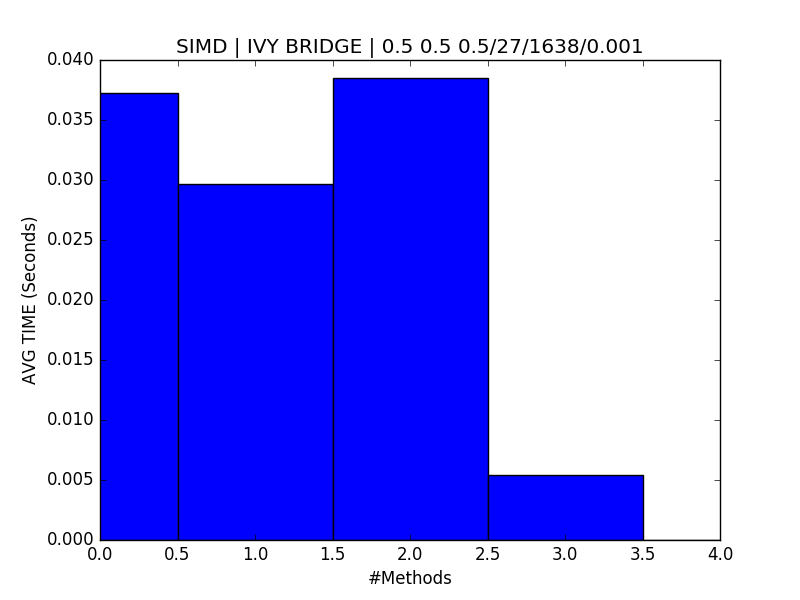
\includegraphics[width=1\textwidth]{experiments/vectorisation/plots/simd.png}
  \end{center}
  \caption{SIMD runtime comparison.}
  \label{figure:triangle_omp}
\end{figure}

\begin{figure}[htb]
  \begin{center}
    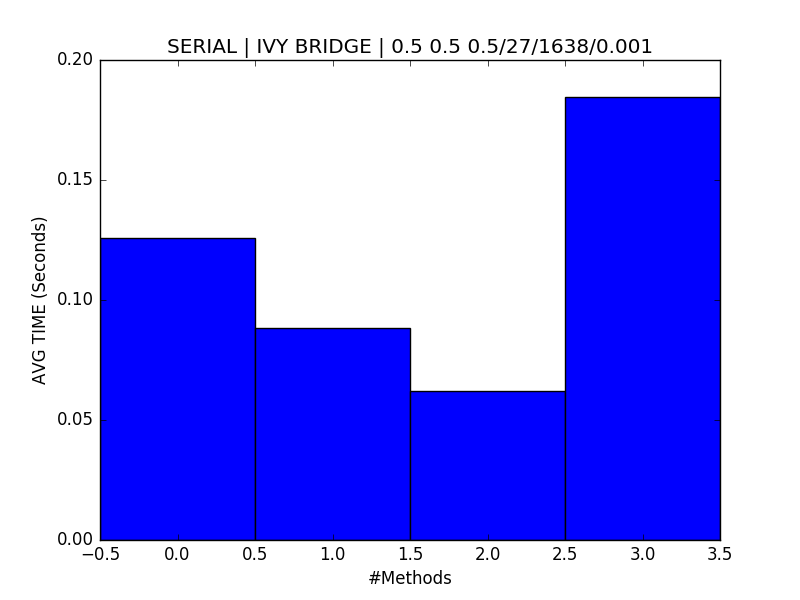
\includegraphics[width=1\textwidth]{experiments/vectorisation/plots/serial.png}
  \end{center}
  \caption{Serial runtime comparison.}
  \label{figure:triangle_omp}
\end{figure}


\clearpage

\subsection{Impact of multiscale grid management}

We start with single core experiments and $diam_{min} = diam_{max} \leq
h_{max}$ where $h_{max}$ is the grid spacing of a regular grid.
Alternatively, we remove the grid completely.
The number of triangle-to-triangle comparisons is reduced dramatically by the
grid which reduces the runtime complexity (Figure \ref{xxx}).
Runtime measurements reflect this fact directly (not shown).
If we release the equality constraint, select $diam_{min} < diam_{max}$ and
allow particles to have an arbitrary diameter between $diam_{min}$ and
$diam_{max}$, we retain the performance compared to the grid-free method.
Once we however use a dynamically adaptive multiresolution grid with inter-grid
particle comparisons, we can reduce the number of triangle-to-triangle
comparisons further. 
From hereon, the characteristic triangle-to-triangle comparison counts from the
multiscale algorithm are used.
For the performance engineering, this is a worst-case choice as the arithmetic
work is minimalised.



Cost
Cache hit rate
Stress on memory subsystem

\section{Conclusion}
\label{section:conclusion}

Works also for FSI. 


Maximale Zeitschrittweitenwahl. Dadurch uebergang zu event-driven scheme.
\section{Conclusion}
\label{section:conclusion}

Works also for FSI. 


Maximale Zeitschrittweitenwahl. Dadurch uebergang zu event-driven scheme.
\section{Acknowledgements}
\label{section:acknowledgements}

This work made use of Durham University's local HPC facilities Hamilton.
We appreciate the support from Intel through Durham's Intel Parallel Computing
Centre (IPCC) which gave me access to latest Intel software.
The work has been sponsored by EPSRC (Engineering and Physical Sciences Research Council) and EDF Energy as part of an ICASE studentship. It also made use of the facilities of N8 HPC provided and funded by the N8 consortium and EPSRC (Grant No. N8HPC \textunderscore DUR \textunderscore TW \textunderscore PEANO). The Centre is co-ordinated by the Universities of Leeds and Manchester. We also thank University of Durham for the supercomputing resources and technical assistance.

\section{Software}
\label{section:software}

All underlying software is free and open source C++ code.
\DeltaSoftware\ is available from \cite{Software:Delta} and offers all the
functionality introduced in Section \ref{section:vectorisation} through
\ref{section:domain-decomposition}.
All spacetree and adaptive mesh refinement routines (Section ref{section:grid}) used in the
present work rely on the framework Peano
\cite{Software:Peano,Weinzierl:2009:Diss,Weinzierl:11:Peano}.
All geometric operations as well as DEM-specific compute kernels however are
independent of Peano and can be used with any other (spacetree-based) software.

We offer \DeltaSoftware\ with single (\texttt{float}) and double
(\texttt{double}).
The accuracy is controlled via a compile flag \texttt{-DiREAL=}.
Subject of study here is exlusively \texttt{double}. 
Studies on reduced accuracy computations are beyond the scope of the present
work.


\bibliographystyle{plain}
\bibliography{./paper}

\appendix

\section{Software}
\label{section:software}

All underlying software is free and open source C++ code.
\DeltaSoftware\ is available from \cite{Software:Delta} and offers all the
functionality introduced in Section \ref{section:vectorisation} through
\ref{section:domain-decomposition}.
All spacetree and adaptive mesh refinement routines (Section ref{section:grid}) used in the
present work rely on the framework Peano
\cite{Software:Peano,Weinzierl:2009:Diss,Weinzierl:11:Peano}.
All geometric operations as well as DEM-specific compute kernels however are
independent of Peano and can be used with any other (spacetree-based) software.

We offer \DeltaSoftware\ with single (\texttt{float}) and double
(\texttt{double}).
The accuracy is controlled via a compile flag \texttt{-DiREAL=}.
Subject of study here is exlusively \texttt{double}. 
Studies on reduced accuracy computations are beyond the scope of the present
work.

\section{Experiment: Two particles}
\label{section:experiment:two-particles}

The present experiments study two particles that bump into each other and then
move away because of the spring dashpot forces.
The two particles are represented by 126 triangles. 
We simulate 15,000 time steps.
A contact is detected first in iteration 9,541 and introduces a force making the
two particles to move away from each other. 
The code however still needs another 5 iterations to make the particles be away
from each other more than $\epsilon=10^{-4}$.
If the two particles are compared, this results in 3,944 triangle-triangle
comparisons.
 
The experiments can be rerun with 
{\footnotesize
\begin{verbatim}
./dem-3d-asserts 0.3 0.1 0.02 two-particles-crash 15000 regular-grid 0.0001 \ 
upon-change 0.0

./dem-3d-asserts 0.3 0.1 0.02 two-particles-crash 15000 adaptive-grid 0.0001 \
upon-change 0.0

./dem-3d-asserts 0.3 0.1 0.02 two-particles-crash 15000 reluctant-adaptive-grid \
0.0001 upon-change 0.0
\end{verbatim}
}

{\bf Regular grid.} We obtain a grid with 1,032 vertices. The first 6,334
iterations, we do not perform any contact detection. The subsequent grid
traversals perform all 3,944 comparisons till iteration 12,503. Starting from
time step 12,504, the particles are far away from each other again and we do not
compare anything anymore.

\begin{center}
  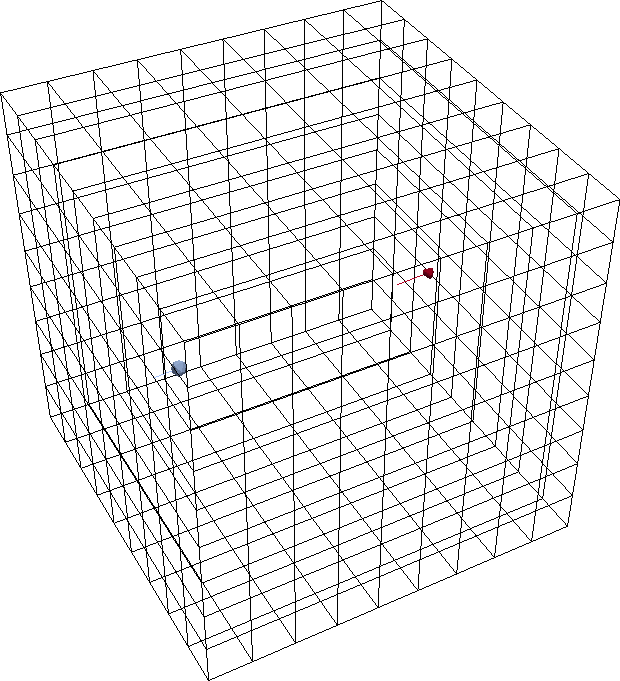
\includegraphics[width=0.3\textwidth]{experiments/two-bodies/visualisation/regular-grid00.png}
  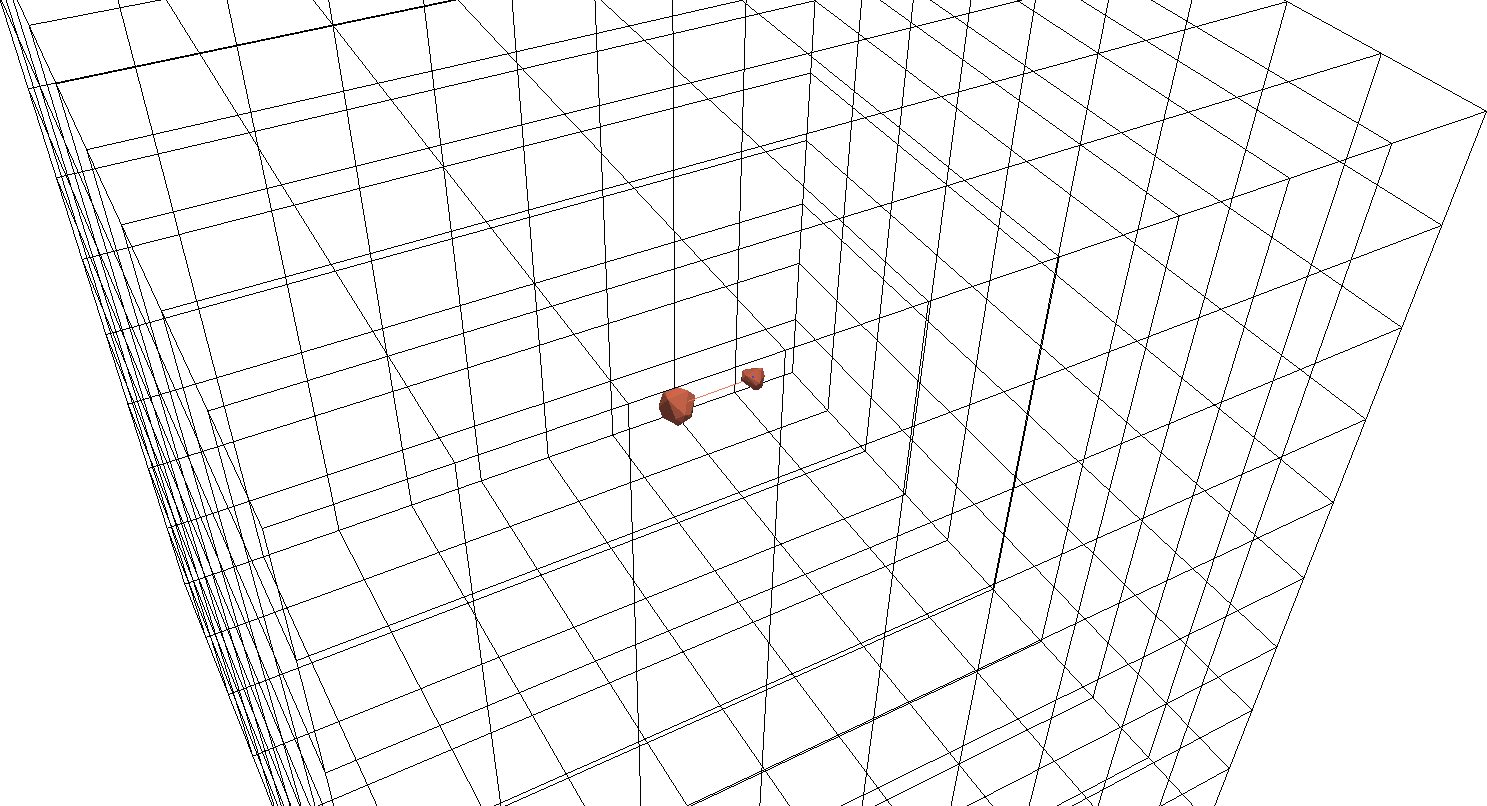
\includegraphics[width=0.3\textwidth]{experiments/two-bodies/visualisation/regular-grid01.png}
  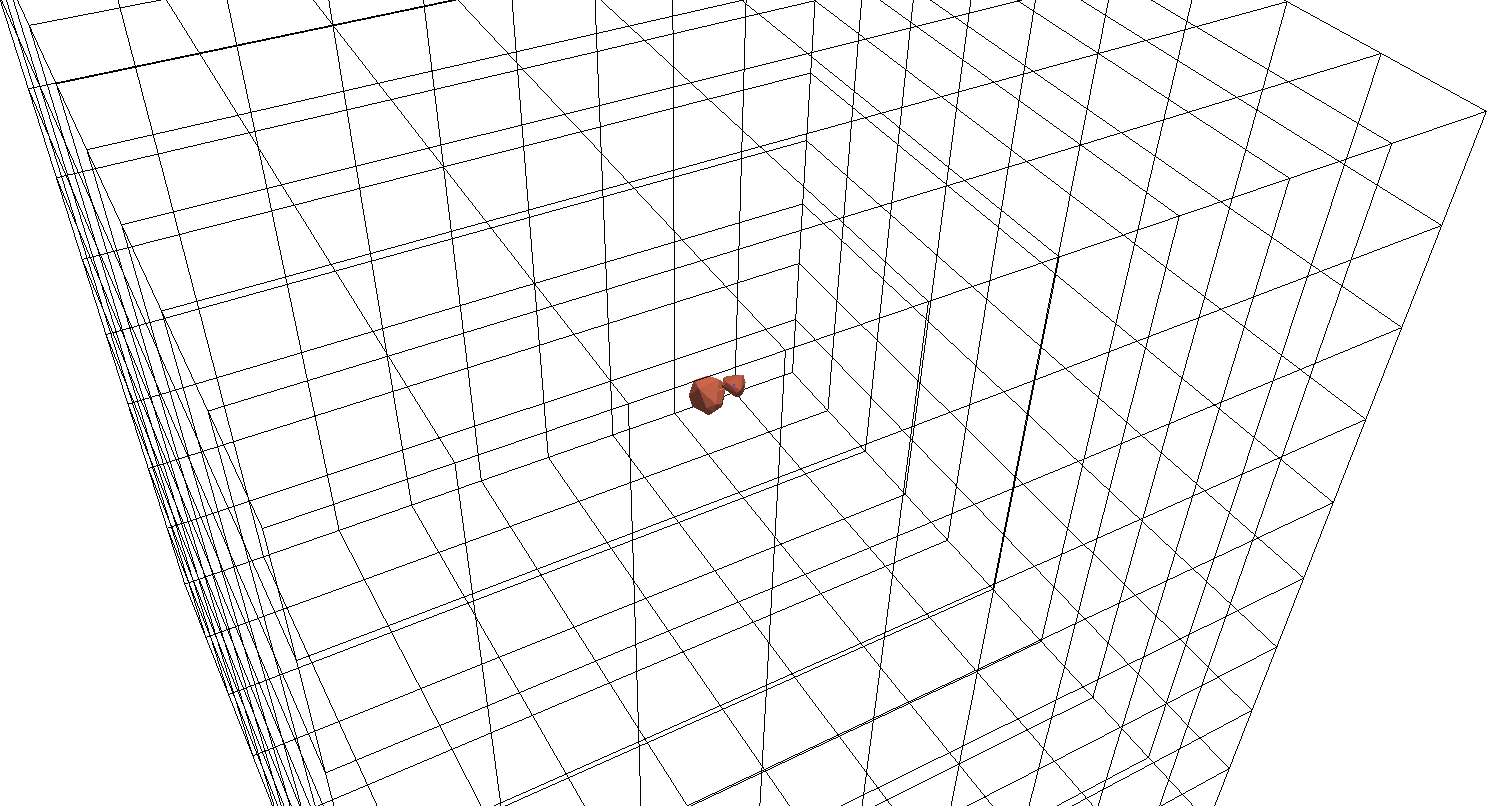
\includegraphics[width=0.3\textwidth]{experiments/two-bodies/visualisation/regular-grid02.png}
\end{center}


{\bf Adaptive grid.} We obtain a grid with 747 vertices. Only few iterations
(when one particle enters a neighbouring region) make the number increase to
980, but these grids are immediately after reduced to 747 again.
The first 8,556 iterations, we do not perform any contact detection. The
subsequent grid traversals perform all 3.944 comparisons.
In iteration 9,539 we detect contact and the particles start to move away
from each other, but we continue to check for further contacts till iteration
10,415.
From here on, the particles are far away from each other again
and we do not compare anything anymore.

% \begin{center}
%   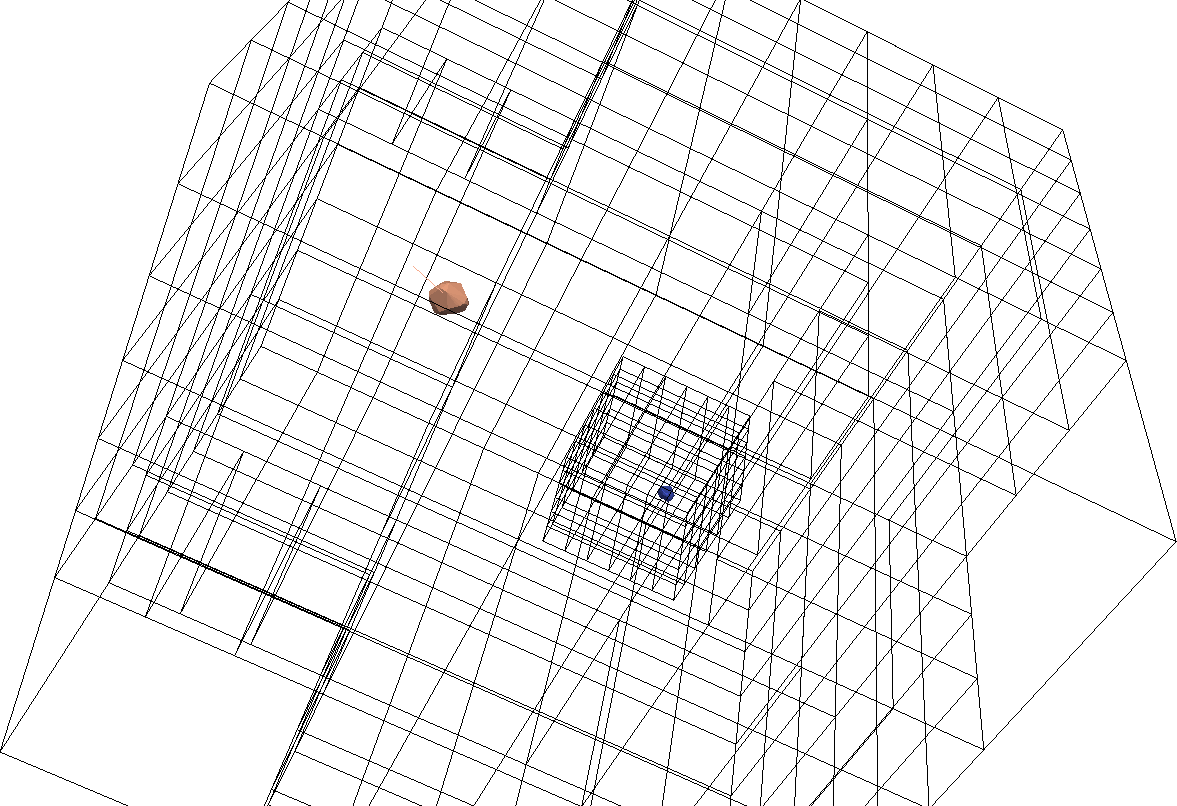
\includegraphics[width=0.3\textwidth]{experiments/two-bodies/visualisation/adaptive-grid00.png}
%   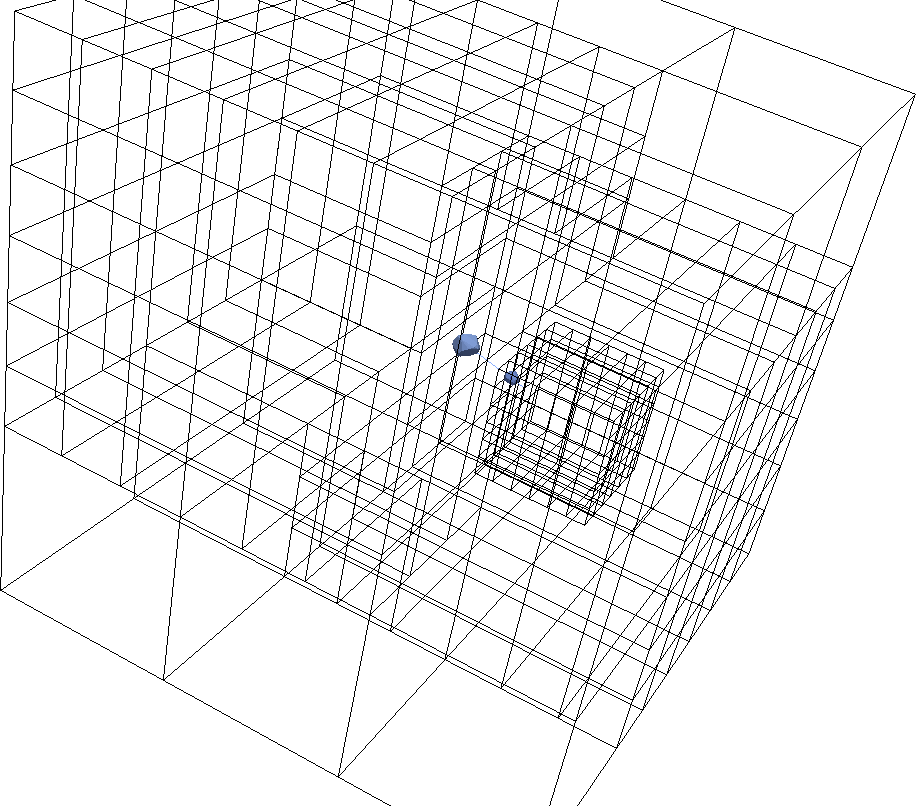
\includegraphics[width=0.3\textwidth]{experiments/two-bodies/visualisation/adaptive-grid01.png}
%   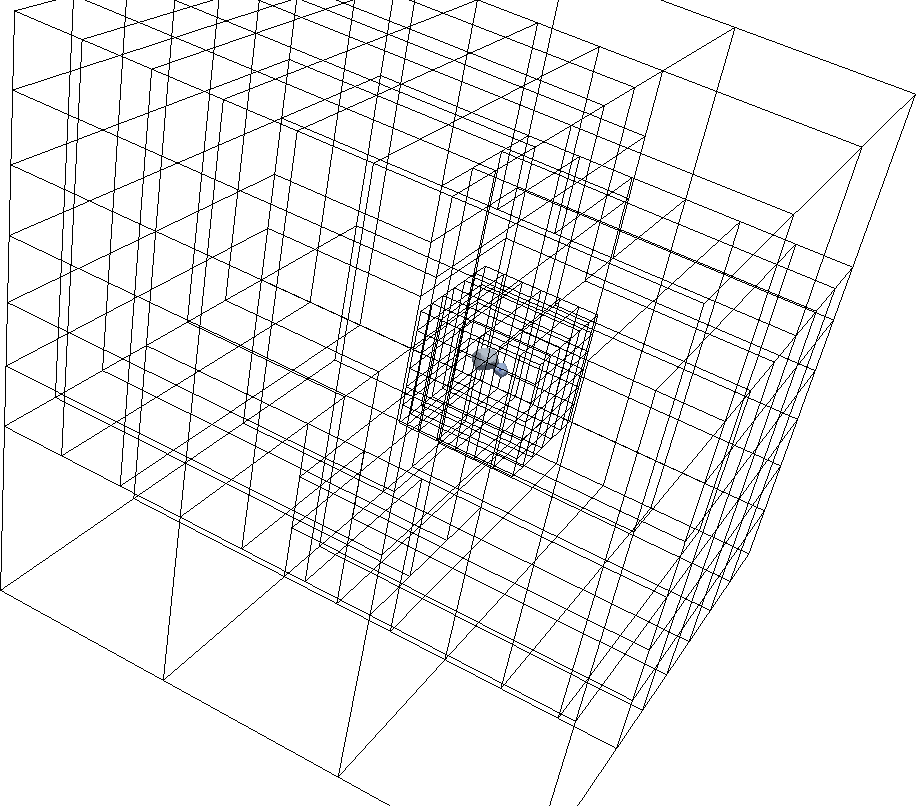
\includegraphics[width=0.3\textwidth]{experiments/two-bodies/visualisation/adaptive-grid02.png}
% \end{center}


{\bf Reluctant adaptive grid.} The reluctant adaptive grid behaves qualitatively
similar to the plain adaptive grid though yields quantitatively a smaller number
of vertices. 
We start from a grid with 498 vertices, i.e.~we do not refine the grid down to
the same fine level as the adaptive approach.
In iteration 6,334, both particles enter the same coarse grid cell and we run
3,944 triangle-triangle comparisions. 
They yield no contact yet.
The reluctant criterion refines the grid that has now 980 vertices starting from
iteration 6,338 on.
The code continues to run without any further comparisons till iteration 8,556
when the particles again are close to each other (close this time w.r.t.~finest
grid level allowed by the particle diameters).
Between iteration 8,557 and 9,533 we continue to run with 980 vertices and
3,944 comparisons.
The code decides to reduce the grid in iteration 9,536 to 747 vertices when the
particles are approach each other within a single cube that is resolved with a
fine grid.
We detects contact in iteration 9,541 after which the particles move away from
each other.
The 747 vertices are preserved and the code continues to run 3,944 comparisons.
In iteration 10,452, the particles are far away from each other. 
No more comparisons are performed from hereon.
In iteration 14,556 the particles are far away from each other, leave the
fine tessellation around the previous contact point and we continue with a
coarser grid of 498 vertices.

%  \begin{center}
%   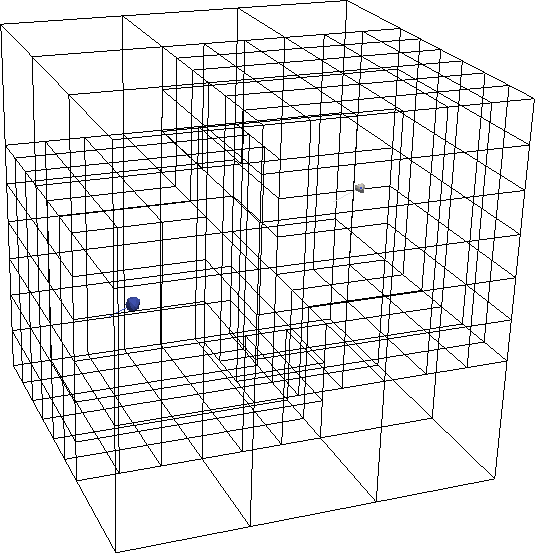
\includegraphics[width=0.3\textwidth]{experiments/two-bodies/visualisation/reluctant-adaptive-grid00.png}
%   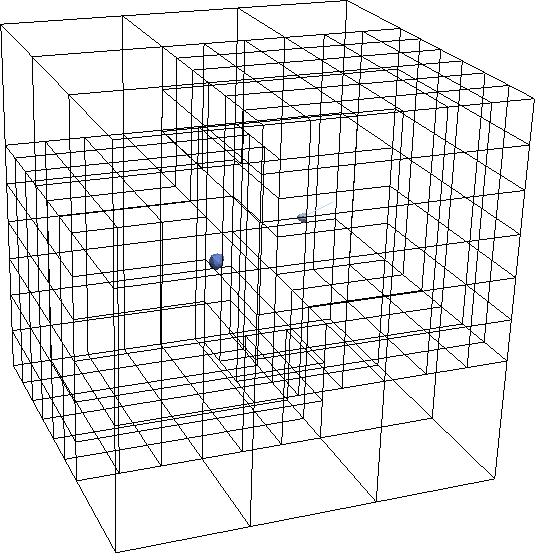
\includegraphics[width=0.3\textwidth]{experiments/two-bodies/visualisation/reluctant-adaptive-grid01.png}\\
%   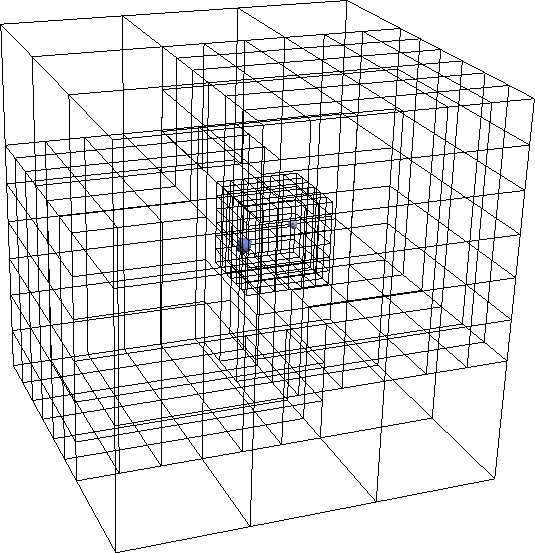
\includegraphics[width=0.3\textwidth]{experiments/two-bodies/visualisation/reluctant-adaptive-grid02.png}
%   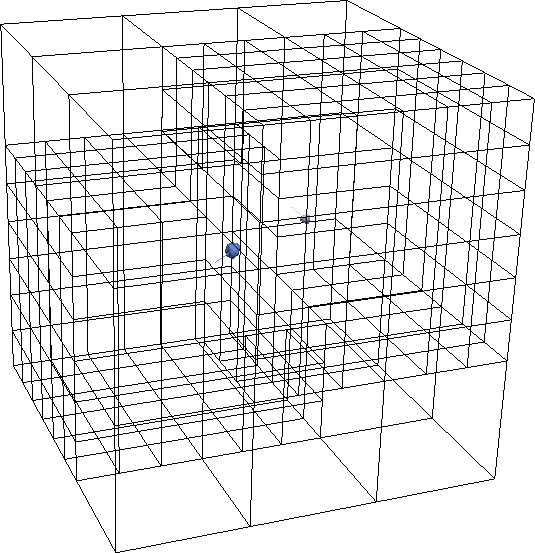
\includegraphics[width=0.3\textwidth]{experiments/two-bodies/visualisation/reluctant-adaptive-grid03.png}\\
%  \end{center}

\section{Experiment: Some comparison statistics}
\label{section:experiment:comparison-statistics}

\begin{center}
  \includegraphics[width=1\textwidth]{experiments/random/no-of-collisions/grid.png}
\end{center}

\begin{center}
 	\includegraphics[width=1\textwidth]{experiments/random/no-of-collisions/adaptive.png}
\end{center}

\begin{center}
  \includegraphics[width=1\textwidth]{experiments/random/no-of-collisions/reluctant.png}
\end{center}

\begin{center}
  \includegraphics[width=1\textwidth]{experiments/random/no-of-collisions/gridG.png}
\end{center}

\begin{center}
  \includegraphics[width=1\textwidth]{experiments/random/no-of-collisions/adaptiveG.png}
\end{center}

\begin{center}
  \includegraphics[width=1\textwidth]{experiments/random/no-of-collisions/reluctantG.png}
\end{center}

\section{Randomised particle generation}
\label{section:randomised-particle-generation}

For our particle generation, we rely on the convex hull algorithm
\cite{mattutis,3,5}.
We place 50 points random on the unit sphere
They act as input to the computation of a convex hull which yields around 60
triangles typically.
Each vertex of the resulting mesh then is scaled with a random scalar from
$[0.75,1]$.
Thus, we obtain distorted particles that do not resemble a sphere and can be
slightly convex.
The resulting mesh is finally suitably dilated and scaled.

\marginpar{\footnotesize KK: Can you please add here two or three pictures from
typical particles?}


\end{document}
